% SIAM Article Template
\documentclass[review,onefignum,onetabnum]{siamonline171218}

% Information that is shared between the article and the supplement
% (title and author information, macros, packages, etc.) goes into
% ex_shared.tex. If there is no supplement, this file can be included
% directly.

\usepackage[utf8]{inputenc} % allow utf-8 input
\usepackage[T1]{fontenc}    % use 8-bit T1 fonts
\usepackage{hyperref}       % hyperlinks
\usepackage{url}            % simple URL typesetting
\usepackage{booktabs}       % professional-quality tables
\usepackage{amsfonts}       % blackboard math symbols
\usepackage{nicefrac}       % compact symbols for 1/2, etc.
\usepackage{microtype}      % microtypography
\usepackage{lipsum}
\usepackage{fancyhdr}       % header
\usepackage{graphicx}       % graphics
\graphicspath{{media/}}     % organize your images and other figures under media/ folder

\usepackage{subfigure}
\usepackage{xcolor}
\usepackage{float}




\usepackage{amsmath}
\usepackage{amssymb}
\usepackage{mathtools}
%\usepackage{amsthm}




\DeclareMathOperator*{\minimize}{\textrm{minimize}}

%%%%%%%%%%%%%%%%%%
%    COMMANDS    %
%%%%%%%%%%%%%%%%%%

\newcommand{\R}{\mathbb{R}}
\newcommand{\expect}{\mathop{\mathbb{E}}}
\newcommand{\observer}{\underset{\lambda,\vartheta}{\mathcal{H}}}
\newcommand{\model}{\underset{\lambda,\vartheta}{\mathcal{M}}}

\newcommand{\twopartdef}[4]{
	\left\{
		\begin{array}{ll}
			#1 & \mbox{if } #2 \\
			#3 & \mbox{if } #4
		\end{array}
	\right.
}

\newcommand{\threepartdef}[6]
{
	\left\{
		\begin{array}{lll}
			#1 & \mbox{if } #2 \\
			#3 & \mbox{if } #4 \\
			#5 & \mbox{if } #6
		\end{array}
	\right.
}





% SIAM Shared Information Template
% This is information that is shared between the main document and any
% supplement. If no supplement is required, then this information can
% be included directly in the main document.


% Packages and macros go here
\usepackage{lipsum}
\usepackage{amsfonts}
\usepackage{graphicx}
\usepackage{epstopdf}
\usepackage{algorithmic}
\ifpdf
  \DeclareGraphicsExtensions{.eps,.pdf,.png,.jpg}
\else
  \DeclareGraphicsExtensions{.eps}
\fi

% Prevent itemized lists from running into the left margin inside theorems and proofs
\usepackage{enumitem}
\setlist[enumerate]{leftmargin=.5in}
\setlist[itemize]{leftmargin=.5in}

% Add a serial/Oxford comma by default.
\newcommand{\creflastconjunction}{, and~}

% Used for creating new theorem and remark environments
\newsiamremark{remark}{Remark}
\newsiamremark{hypothesis}{Hypothesis}
\crefname{hypothesis}{Hypothesis}{Hypotheses}
\newsiamthm{claim}{Claim}

% Sets running headers as well as PDF title and authors
\headers{SCENE-Net}{D. Lavado, C. Soares, and A. Micheletti}

% Title. If the supplement option is on, then "Supplementary Material"
% is automatically inserted before the title.
\title{
Low-Resource White-Box Semantic Segmentation of Supporting Towers on 3D Point Clouds via Signature Shape Identification
    % \thanks{Submitted to the editors DATE.
    %     \funding{This work was funded by the Fog Research Institute under contract no.~FRI-454.}
    % }
}



\author{Diogo Lavado\footnotemark[1], Cláudia Soares\thanks{NOVA School of Science and Technology, Lisbon 
  (\email{d.lavado@campus.fct.unl.pt}, \email{claudia.soares@fct.unl.pt}).}
\and Alessandra Micheletti\footnotemark[2], Giovanni Bocchi\thanks{University of Milan, Milan
  (\email{alessandra.micheletti@unimi.it}, \email{giovanni.bocchi1@unimi.it}).}
\and Alex Coronati\footnotemark[3], Manuel Pio\thanks{EDP NEW, Lisbon
  (\email{alex.coronati@edp.pt}, \email{manuelpio.silva@edp.pt}).}
\and Patrizio Frosini\thanks{University of Bologna, Bologna
  (\email{patrizio.frosini@unibo.it}).}
}
% \author{Dianne Doe\thanks{Imagination Corp., Chicago, IL 
%   (\email{ddoe@imag.com}, \url{http://www.imag.com/\string~ddoe/}).}
% \and Paul T. Frank\thanks{Department of Applied Mathematics, Fictional University, Boise, ID 
%   (\email{ptfrank@fictional.edu}, \email{jesmith@fictional.edu}).}
% \and Jane E. Smith\footnotemark[3]}

\usepackage{amsopn}
\DeclareMathOperator{\diag}{diag}


%%%% HELPER CODE FOR DEALING WITH EXTERNAL REFERENCES ON OVERLEAF
% (from an answer by cyberSingularity at http://tex.stackexchange.com/a/69832/226)
%%%
\makeatletter
\newcommand*{\addFileDependency}[1]{% argument=file name and extension
  \typeout{(#1)}% latexmk will find this if $recorder=0 (however, in that case, it will ignore #1 if it is a .aux or .pdf file etc and it exists! if it doesn't exist, it will appear in the list of dependents regardless)
  \@addtofilelist{#1}% if you want it to appear in \listfiles, not really necessary and latexmk doesn't use this
  \IfFileExists{#1}{}{\typeout{No file #1.}}% latexmk will find this message if #1 doesn't exist (yet)
}
\makeatother

\newcommand*{\myexternaldocument}[1]{%
    \externaldocument{#1}%
    \addFileDependency{#1.tex}%
    \addFileDependency{#1.aux}%
}
%%% END HELPER CODE

%%% Local Variables: 
%%% mode:latex
%%% TeX-master: "ex_article"
%%% End: 


% Optional PDF information
\ifpdf
\hypersetup{
  pdftitle={Low-Resource White-Box Semantic Segmentation of Supporting Towers on 3D Point Clouds via Signature Shape Identification},
  pdfauthor={D. Lavado, C. Soares and A. Micheletti}
}
\fi

% The next statement enables references to information in the
% supplement. See the xr-hyperref package for details.

%% Use \myexternaldocument on Overleaf
\myexternaldocument{ex_supplement}

% FundRef data to be entered by SIAM
%<funding-group>
%<award-group>
%<funding-source>
%<named-content content-type="funder-name"> 
%</named-content> 
%<named-content content-type="funder-identifier"> 
%</named-content>
%</funding-source>
%<award-id> </award-id>
%</award-group>
%</funding-group>

\begin{document}


\maketitle

% REQUIRED
\begin{abstract}
%Machine Learning is now changing the game for real-world applications.
Research in 3D semantic segmentation has been increasing performance metrics, like the IoU, by scaling model complexity and computational resources, leaving behind researchers and practitioners that (1) cannot access the necessary resources and (2) need transparency on the model decision mechanisms.
%
%High-risk tasks require human-auditable models that provide insight into their decision-making process to non-expert users, and that can be efficient for both a small, noisy data regime and regular hardware.
%
In this paper, we propose SCENE-Net, a low-resource white-box model for 3D point cloud semantic segmentation of pole-like objects. 
SCENE-Net identifies signature shapes on the point cloud via group equivariant non-expansive operators (GENEOs), providing intrinsic geometric interpretability.
Our model serves as a proof-of-concept that GENEOs can be used to build learning agents that are interpretable, robust to noisy labeling, and resource-efficient.
%
We apply SCENE-Net to the challenging detection of power line supporting towers in power grids---a key task in preventing forest fires and power outages.
Our training time on a laptop is 85~min, and our inference time is 20~ms. SCENE-Net has 11 trainable geometrical parameters,
like the radius of a ball, and a Precision gain of 38\% against a comparable CNN with 2190 parameters.
SCENE-Net requires less data to train and shows robustness to data imbalance. 
With this paper, we release our code implementation: \url{https://github.com/dlavado/scene-net}.
\end{abstract}

% REQUIRED
\begin{keywords}
    3D Semantic Segmentation, Point Clouds, Group Equivariant Non-Expansive Operators, White-Box Models, Power Grids
\end{keywords}

% REQUIRED
\begin{AMS}
  68T45, % Machine vision and scene understanding 
  46N10, % Applications in optimization, convex analysis, mathematical programming, economics
  58K70  % Symmetries, equivariance
\end{AMS}

\section{Introduction}\label{sec:intro}
% Structure
% paragraph 1: Broad problem
% paragraph 2: more specific
% paragraph 3: more more specific
% paragraph 4: more more more specific
% paragraph 5: Wrap up the story
% When citing, refer to the relevant contribution to our story 

\begin{figure}[t]
\centering
\subfigure[TS40K Sample]{\label{fig:intro_input}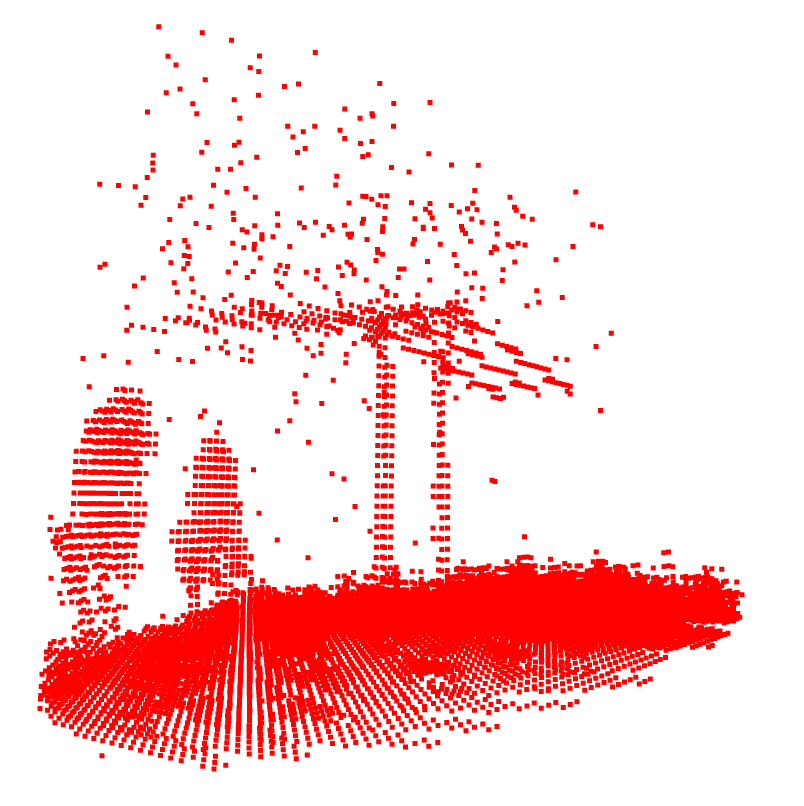
\includegraphics[width=.29\columnwidth]{s37.png}}
%
\subfigure[SCENE-Net]{\label{fig:intro_gnet}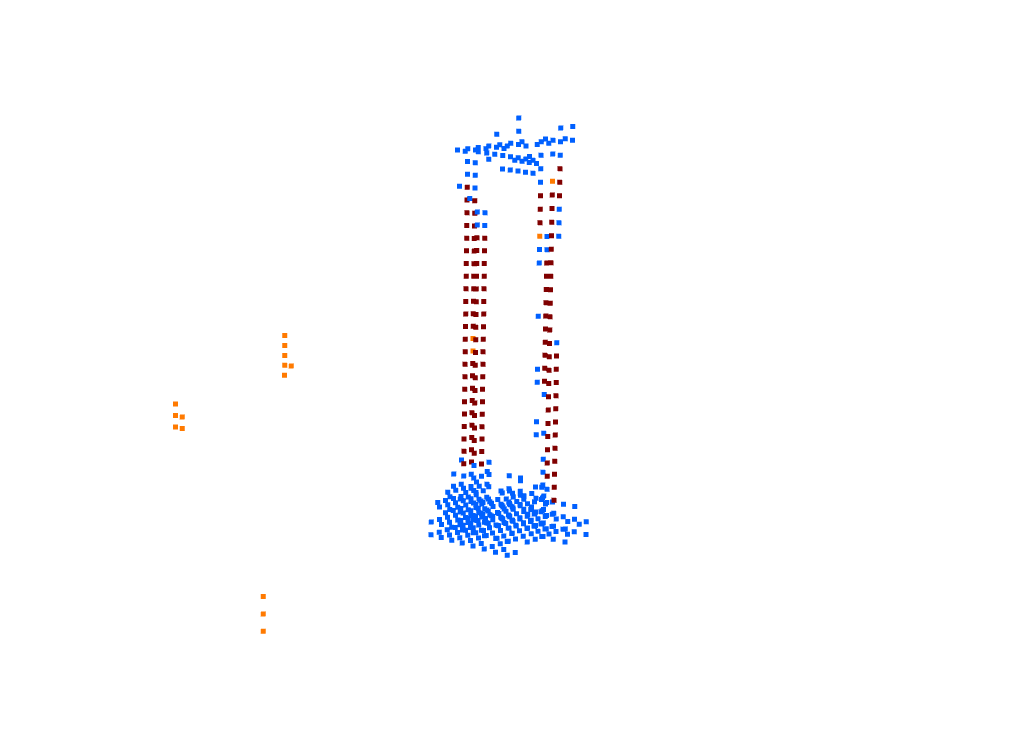
\includegraphics[width=.37\columnwidth]{gnet_s37.png}}
%
\subfigure[Baseline CNN]{\label{fig:intro_cnn}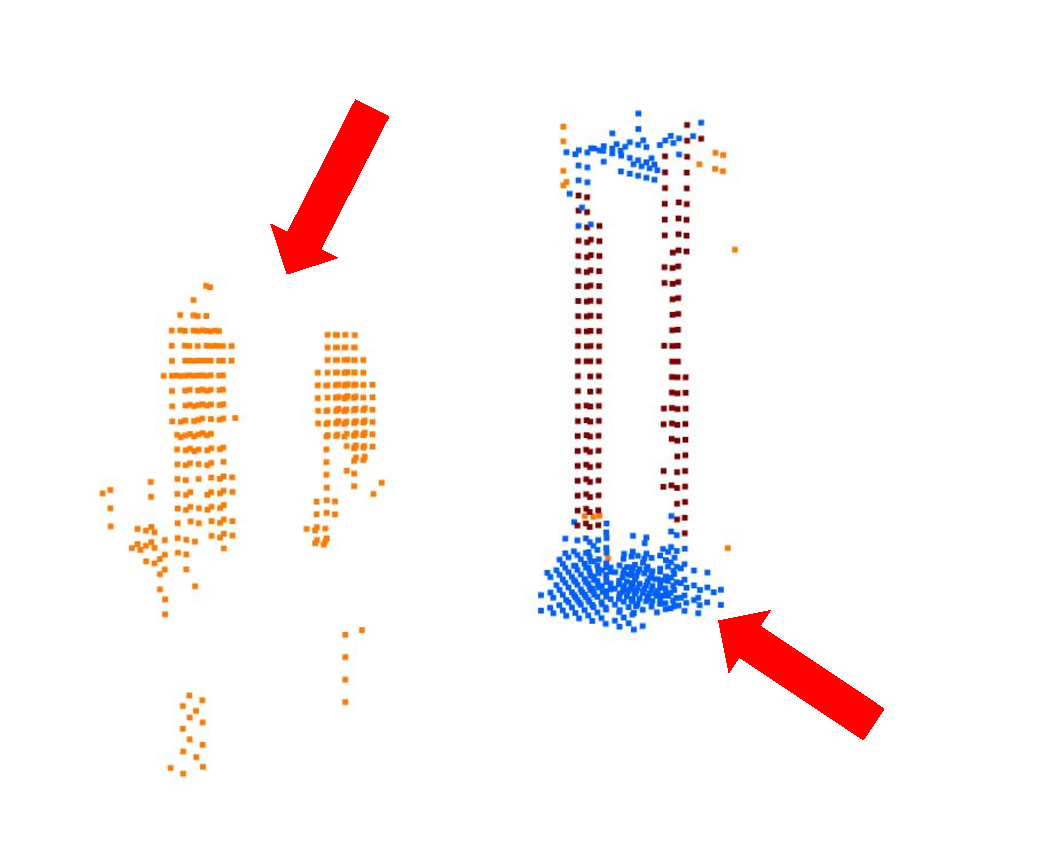
\includegraphics[width=.32\columnwidth]{cnn_s37.pdf}}
%
\subfigure
{\centering
\includegraphics[width=.5\columnwidth]{color_code_v2.pdf}}
\caption{Signature shapes for power line supporting tower detection.
For our TS40K sample shown in (a), SCENE-Net accurately detects the body of the tower (b), while a comparable CNN has a large false positive area in the vegetation (c). Our model is interpretable with 11 trainable geometric parameters whereas the CNN has a total of 2190 parameters. The ground and power lines are mislabeled in the ground truth}
\label{fig:intro_fig}
\end{figure}

%
% paragraph 1: Broad problem
% First sentence: every reader of the paper should understand this sentence. Make it compelling. State the broad problem. Move from broad to narrow.


Powerful Machine Learning (ML) algorithms applied to critical applications, such as autonomous driving or environmental protection, highlight the importance of (1) ease of implementation for non-tech organization, entailing data efficiency and general-purpose hardware, and (2) transparent models regarding their decision-making process, thus ensuring a responsible deployment~\cite{lipton2018mythos,guidotti2018survey, doshi2017towards}. 
%
% The performance of black-box models on a test set is often used as a confidence measure for their usability in real-world scenarios, however, such performance does not consider out-of-distribution data and provides no reasoning behind the predictions of models that might be essential in high-risk tasks.
%
% Existing black-box models , while achieving high performance on test sets, do not provide insight into their reasoning, and are not robust to out-of-distribution data.
%
Most methods in Explainable AI (XAI) provide \textit{post hoc} explanations to black-box models (i.e., algorithms unintelligible to humans). However, these are often limited in terms of their model fidelity~\cite{lipton2018mythos,rudin2019stop}, that is, they provide explanations for the predictions of the underlying model (e.g., heatmaps~\cite{Chefer_2021_CVPR,voita2019analyzing} and input masks~\cite{ribeiro2016should,fong2017interpretable}), instead of providing a mechanistic understanding of its inner-workings.
%
% Explainable methods address this issue by providing \textit{post hoc} reasoning for existing black-box models (i.e., algorithms unintelligible to humans), but these cannot guarantee perfect fidelity with respect to the inner workings of the original model~\cite{lipton2018mythos,rudin2019stop}, instead, they provide possible explanations (e.g., heatmaps~\cite{Chefer_2021_CVPR,voita2019analyzing} and input masks~\cite{ribeiro2016should,fong2017interpretable}) that do not provide insights into what the black-box is actually computing.
%
%
Conversely, intrinsic interpretability methods (i.e., white-box models) provide an
understanding of their decisions through their architecture
and parameters~\cite{rudin2019stop}.
%
Transparency is achieved by enforcing constraints that reflect domain knowledge and simple designs~\cite{lipton2018mythos,chen2020concept}, which can result in a loss in performance when compared to complex black-boxes.

We propose a novel white-box model, \textbf{SCENE-Net}, that provides intrinsic geometric interpretability by leveraging on group equivariant non-expansive operators (GENEOs)~\cite{GENEO19,GENEO21}. Unlike traditional interpretable models, GENEOs are complex observers parameterized with meaningful geometric features.
%
% This allows for resource-efficient training and robustness to noisy labeling and data imbalance, even in small datasets.
%
%The interpretability of SCENE-Net comes through its formal description as a set of operations (GENEOs) acting on input data, observing signature shapes relevant to the task at hand. 
%
% GENEOs are operators that transform data while preserving a pre-defined set of meaningful features.
% In this framework, ML models are formally described as a set of operations acting on the input data that observe properties we aim to identify,  
% which allows us to embed domain knowledge into a learning model and drastically decrease the number of trainable parameters while ensuring strong geometric interpretability.
% , which is incompatible with the current trend in Deep Learning (DL) where models scale up in both parameters and data requirements to boost performance, with recent language models being a prime example~\cite{chowdhery2022palm}.
% %
% % Additionally, current Deep Learning (DL) methods are quickly scaling up in terms of both complexity with convoluted architectures and in computational and data requirements, with recent language models being a prime example.
% %
% % This induces an environment where training state-of-the-art models is out of reach for most researchers, scholars, and even traditional institutions, such as utilities.
% %
% Thus, the development of DL strategies in high-risk scenarios is often handicapped by the lack of transparency of black-box models and the lack of resources (data and computing power) to employ recent models.
% In this work we introduce \textbf{SCENE-Net}, 
% an intrinsically interpretable 3D point cloud semantic segmentation framework identifying signature shapes with group equivariant non-expansive operators (GENEOs)~\cite{GENEO19,GENEO21} that allows for resource-efficient training and exhibits robustness to noisy labeling and data imbalance even in small datasets.
%
% GENEOs are operators that transform data while preserving a pre-defined set of meaningful features.
% %
% In this framework, ML models are formally described as a set of operations acting on the input data that observe properties we aim to identify,  
% %
% which allows us to embed domain knowledge into a learning model and drastically decrease the number of trainable parameters while ensuring strong geometric interpretability.
%
In our case, task dependency comes as a collaboration of Machine Learning and electrical utility teams to transparently segment
power line supporting towers on 3D point clouds to inspect extensive power grids automatically.
%
Electrical grid operators have the critical job of assessing the risk of contact between the power grid and its environment to prevent failures and forest fires. These grids spread over countries and even continents, thus making careful inspection an important and challenging problem. 
%
Often, this task is based on LiDAR large-scale point clouds with high-point density, no sparsity, and no object occlusion. However, the captured point clouds are quite extensive and mostly composed of rural areas. 
These data are different from large urban datasets for autonomous driving~\cite{Semantic3D,SemKITTI} due to the point of view, point density, occlusion, and extension.
%
To bootstrap this work, we created a labeled dataset of 40~000~Km of rural and forest terrain, and the \textbf{T}ransmission \textbf{S}ystem, named \textbf{TS40K}. 
%
These point clouds show noisy labels and class imbalance (see Appendix~\ref{sec:ts40k} for details), and SCENE-Net is robust to labeling noise as it encodes the geometric properties we need to detect. 


Moreover, practitioners in high-risk tasks, such as autonomous driving and power grid inspection, are often limited in terms of resources, namely computational power and available data, to train and deploy state-of-the-art models~\cite{muhammad2020deep,alzubaidi2021review}.
This clashes with the current trend in DL to scale up models in both complexity and needed resources in order to maximize performance, for example, state-of-the-art 3D semantic segmentation models~\cite{thomas2019kpconv,tang2020searching,xu2021rpvnet,yan2021sparse,yan20222dpass} follow this trend.
%
Our model, SCENE-Net, maintains a simple design conventional to white-boxes (it is composed of 11 trainable parameters) that allows for resource-efficient training while taking advantage of powerful Deep Learning (DL) strategies, such as convolutions.
%
By assessing our model on the SemanticKITTI benchmark~\cite{SemKITTI}, we show that SCENE-Net achieves performance on-par with state-of-the-art methods in pole segmentation.
% Nevertheless, we provide a quantitative comparison of SCENE-Net on the SemanticKITTI benchmark~\cite{SemKITTI} to 

%Classes like the ground, cannot be easily removed, due to terrain irregularity. 
%Power line supporting towers make up less than 1\% of the overall point clouds, and noisy labeling is a major issue: patches of ground incorrectly classified are 40\% of tower 3D points.

%In order to provide operators with an accurate coordinate prediction of power line supporting towers, as well as measure the risk of contact between towers and the environment, we propose their detection via 3D semantic segmentation.
% We propose the detection of power line supporting towers via 3D semantic segmentation in order to provide TSOs with an accurate coordinate prediction and make available the contact risk prediction with the environment.
%
% A possible approach is to employ 3D semantic segmentation methodologies.
% %
% State-of-the-art represents 3D scenes as volumetric grids~\cite{wu20153d,maturana2015voxnet} and as 3D point clouds~\cite{qi2017pointnet,qi2017pointnet++,thomas2019kpconv}.
% %
% Volumetric methods allow for the use of global feature descriptors, such as 3D convolutions. But are restricted in resolution due to the cubic growth of computational complexity and memory footprint.
% %
% % 3D Point Clouds are the preferred medium to represent 3D environments, as they offer a compact and fine-detailed depiction of the 3D data. However, they also introduce challenges to ML models, namely  heterogeneous density, lack of structure and permutation invariance.
% 3D point clouds offer a compact and fine-detailed depiction of 3D scenes.
% However, they also introduce challenges to ML models, namely heterogeneous density, lack of structure and permutation invariance. 
% %
% State-of-the-art methods~\cite{qi2017pointnet++,thomas2019kpconv,AF2S3Net,Cylinder3D,yan20222dpass,xu2021rpvnet} increased their complexity in order to address these challenges and yield good performance on real-life scenarios, such as autonomous driving.
% %
% These models have millions of trainable parameters, non-trivial amount of training time and specific hardware requirements.
% Additionally, most proposals are tailored to boost performance in urban settings (e.g., Semantic3D~\cite{Semantic3D}, SensatUrban~\cite{SensatUrban} and SemanticKITTI~\cite{SemKITTI}), where data are sparse, objects are often occluded and may demonstrate anisotropy w.r.t. density. 
%
%Despite the promising performance on urban scenarios, these methodologies on outdoor non-urban environments with different data properties such as severe data imbalance, to the best of our knowledge, still remains to be studied.
%

Our main contributions are:
\begin{itemize}
   
    \item SCENE-Net is the first white-box model for 3D semantic segmentation on large-scale landscapes, including non-urban environments (Section~\ref{sec:method});
   
    \item The architecture of SCENE-Net has fewer trainable parameters than traditional methods and is resource-efficient in both data and computational requirements (Section~\ref{sec:results-time-efficiency});

    \item Empirically, SCENE-Net is intrinsically and posthoc interpretable and robust under noisy labels, with au par IoU (Section~\ref{sec:results-interpretability});
    
    \item We present TS40K, a new 3D point cloud dataset covering 40 000 Km of non-urban terrain, with more than 9000 million 3D points (details in Appendix~\ref{sec:ts40k});
    % \item As GENEOs are continuous observer functions, SCENE-Net is independent from input and kernel voxelized shapes. I.e., it can change the kernel shape after training. SCENE-Net's kernel-size is fine-tuned after training to boost its performance
    %is trained with low-resolution kernels achieves same or better performance in high-resolution inference
    %(Section~\ref{sec:results-resolution}).
\end{itemize}

\section{Related Work}
\label{sec:related-work}

\subsection{Point Cloud Semantic Segmentation}
% Here I would give a brief contextualization of 3D semantic segmentation; talking about the first pioneer PointNet and the advancements in 3D convolutions applied to points clouds via voxel-based and point-based methods. This is standard for papers in this research field.
Processing point clouds is a challenging task due to their unstructured nature and invariance to permutations. 
%Approaches can be divided in three groups: multi-view-based, voxel-based and point-based. Multi-view-based methods project point clouds onto 2D planes~\cite{MultiViewLawin} or spherical representations~\cite{wu2018squeezeseg} so that 2D CNNs can be employed~\cite{tatarchenko2018tangent,iandola2016squeezenet}.
%
Voxel-based strategies endow point clouds with structure in order to apply 3D convolutions~\cite{long2015fully,rethage2018fully,tchapmi2017segcloud}. However, memory footprint is too large for high-resolution voxel grids, while low resolution entails information loss. 
%
Subsequent methods try to answer these issues by employing sparse convolutions~\cite{graham20183d,su2018splatnet} and octree-based CNNs~\cite{wang2017cnn,le2018pointgrid}.
%
Point-based models take point clouds directly as input.
The work of PointNet~\cite{qi2017pointnet} and PointNet++~\cite{qi2017pointnet++} inspired the use of point sub-sampling strategies with feature aggregation techniques to learn local features on each sub-point~\cite{hu2020randla,xu2020geometry}.
%
Convolution-based methods~\cite{hua2018pointwise,li2018pointcnn,wu2019pointconv,thomas2019kpconv,Cylinder3D} demonstrate good performance on 3D semantic segmentation benchmarks, such as \textit{SemanticKITTI}~\cite{SemKITTI} and SensatUrban~\cite{SensatUrban}.
%
Following this strategy, recent methods exploit multi-representation fusion, i.e, they combine different mediums (voxel grids, raw point clouds, and projection images) to boost feature retrieval~\cite{AF2S3Net,tang2020searching,xu2021rpvnet,yan20222dpass} and achieve top performance on the above benchmarks.
%
While voxel-based methods are computationally expensive due to 3D convolutions on high-resolution voxel grids, point-based strategies have to use costly neighbor searching to extract local information.
We propose a voxel-based architecture that is time-efficient with high-resolution voxel grids, with shapes of $64^3$ and $128^3$.
Moreover, learning from imbalanced and noisy data is still a challenging task in point cloud segmentation~\cite{guo2020deep},
%
SCENE-Net is interpretable and robust to these conditions.



\subsection{Power line segmentation from 3D point clouds.} 
Power line inspection is generally performed by on-site maintenance personnel and manned helicopters that examine the power grid with portable devices or the naked eye. 
%
These methods are costly, inefficient, and demanding for staff. 
%
Thus, process automation is crucial for operators.
%
To this end, unmanned aerial vehicles (UAVs) carrying LiDAR sensors are deployed to scan the power grid and capture a 3D point cloud representation of the environment.
%
In the work~\cite{ding2021electric}, the authors combine SLAM algorithms with multi-sensor data to patrol the electrical grid with UAVs. This method employs a multi-view-based approach to point cloud segmentation, so the 3D reconstructions from 2D raster maps usually introduce information loss and decrease in accuracy.
%
Alternative methods project point clouds onto the $xy$-plane in order to cluster them~\cite{guo2019research} to segment power lines. This approach does not consider ground and irregular terrain and focuses on segmenting incomplete power lines.
%
Other methods take advantage of fine-grained elevation statistics of the original point cloud and $xy$-plane projections~\cite{tao2019study}.
%
The proposals above focus on the segmentation of high-voltage power lines and disregard their supporting towers.
%
By incorporating prior knowledge, our proposal segments supporting towers of any voltage. Not only are these structures also subject to inspections, but they serve as a point of reference for the location of power lines. 
In addition, by taking into account raw 3D scenes, other scene elements, such as vegetation, can be segmented to assess the risk of contact between the power grid and the environment.

% L. Ding, J. Wang and Y. Wu, "Electric power line patrol operation based on vision and laser SLAM fusion perception," 2021 IEEE 4th International Conference on Automation, Electronics and Electrical Engineering (AUTEEE), 2021, pp. 125-129, doi: 10.1109/AUTEEE52864.2021.9668784.
%
% T. Guo et al., "Research on Point Cloud Power Line Segmentation and fitting algorithm," 2019 IEEE 4th Advanced Information Technology, Electronic and Automation Control Conference (IAEAC), 2019, pp. 2404-2409, doi: 10.1109/IAEAC47372.2019.8997632.
%
% G. Tao et al., "Study on segmentation algorithm with missing point cloud in power line," 2019 IEEE 3rd Advanced Information Management, Communicates, Electronic and Automation Control Conference (IMCEC), 2019, pp. 1895-1899, doi: 10.1109/IMCEC46724.2019.8983925.


\subsection{Explainable Machine Learning}
% Chen, Zhi, Yijie Bei, and Cynthia Rudin. "Concept whitening for interpretable image recognition." Nature Machine Intelligence 2.12 (2020): 772-782.
%
%Barbiero, Pietro, et al. "Entropy-based logic explanations of neural networks." Proceedings of the AAAI Conference on Artificial Intelligence. Vol. 36. No. 6. 2022.
%
%

Explainability is a crucial aspect of ML methods in high-stakes tasks such as autonomous driving~\cite{lipton2018mythos,guidotti2018survey,doshi2017towards}.
%
Two main approaches have been proposed in the literature: \textit{post hoc} explainability, and intrinsic interpretability.
%
\textit{Post hoc} methods, such as LIME~\cite{ribeiro2016should}, meaningful perturbations~\cite{fong2017interpretable}, anchors~\cite{ribeiro2018anchors}, and ontologies~\cite{leite21}, are applied to trained black-box models and provide instance-based explanations that correlate model predictions to the given input. 
%
These methods are model-agnostic, and thus more flexible, but they often lack mechanistic cause-effect relations and have a limited understanding of feature importance~\cite{rudin2019stop}.
%
For instance, a dog image and random noise may generate similar importance heatmaps for the same class with the LIME method~\cite{rudin2019stop}.
%
Moreover, they introduce computational overhead, which may limit their application in real-world scenarios with complex black-box models, such as in the 3D semantic segmentation task.
%
In contrast, intrinsic interpretability methods provide an understanding of their decisions through their architecture and parameters~\cite{rudin2019stop}. Decision trees and linear regression are examples of white-box models. However, transparency is usually achieved by imposing domain constraints and simple designs, which implies limited performance compared to deep neural networks.
%
Recent advances in interpretable techniques, such as concept whitening~\cite{chen2020concept} and interpretable CNNs~\cite{Zhang_2018_CVPR}, have shown that interpretability does not have to imply performance loss. 
However, these methods provide evidential interpretability, that is, they offer intrinsic explanations to model predictions that are still linked to human interpretations and may imply an evidential correlation, but not causation.

We propose a white-box model, SCENE-Net, with intrinsic geometric interpretability that is not subject to human interpretation.
SCENE-Net analyzes the input 3D space according to prior knowledge of the geometry of objects of interest, which is encoded in functional observers and whose parameters are fine-tuned during training. These observers encode high-level geometrical concepts.
Thus, our predictions exhibit direct mechanistic cause-effect w.r.t. the learned observers. 
SCENE-Net maintains a simple model design in high-level mathematical operations while taking advantage of DL complex convolutional kernels. 

% SCENE-Net offers a unique combination of interpretability, performance, and causality, making it a valuable tool for high-risk tasks and other applications in which interpretability is a crucial requirement.

\section{Group Equivariant Non-Expansive Operators (GENEOs)} 

GENEOs are the building blocks of a mathematical framework~\cite{GENEO19} that formally describes machine learning agents as a set of operators acting on the input data. 
These operators provide a measure of the world, just as CNN kernels learn essential features to, for instance, recognize objects. 
%
Such agents can be thought of as observers that analyze data. They transform it into higher-level representations while respecting a set of properties (i.e., a group of transformations).
%
%For instance, applying planar translations to supporting towers preserves the information they carry. 
An appropriate observer transforms data in such a way that respects the right group of transformations, that is, it commutes with these transformations. Formally, we say that the observer is \textit{equivariant} with respect to a group of transformations. 
%
The framework takes advantage of topological data analysis (TDA) to describe data as topological spaces. 
Specifically, a set of data $X$ is represented by a topological space $\Phi$ with admissible functions $\varphi \colon X\to \R^3$. $\Phi$ can be thought of as a set of admissible measurements that we can perform on the measurement space $X$. For example, images can be seen as functions assigning RGB values to pixels. 
This not only provides uniformity to the framework but also allows us to shift our attention from raw data to the space of measurements that characterizes it.
%
Now that the input data is well represented, let us introduce how the framework defines prior knowledge. 
Data properties are defined through maps from $X$ to $X$ that are $\Phi$-preserving homeomorphisms. 
%Two spaces are considered topologically equal if they present a homeomorphism between them.
That is, the composition of functions in $\Phi$ with such homeomorphisms produces functions that still belong to $\Phi$.
% Meaning that such functions do not spoil the properties of $\Phi$ when applied and $X$ remains topologically the same.
Therefore, we can define a group $G$ of $\Phi$-preserving homeomorphisms, representing a group of transformations on the input data for which we require equivariance to be respected.
In other words, $G$ is the group of properties that we chose to enforce equivariance w.r.t. the geometry in the original data. 
It is through $G$ that we embed prior knowledge into a GENEO model. Following the previous example, planar translations can define a subgroup of $G$.

Let us consider the notion of a \textit{perception pair} $(\Phi, G)$: it is composed of all admissible measurements $\Phi$ and a subgroup of $\Phi$-preserving homeomorphisms $G$.
%
\begin{definition}[Group Equivariant Non-Expansive Operator (GENEO)]
Consider two perception pairs $(\Phi, G)$ and $(\Psi, H)$ and a homomorphism $T\colon G \to H$. A map $F\colon \Phi \to \Psi$ is a group equivariant non-expansive operator if it exhibits equivariance:
\begin{equation}
    \forall \varphi \in \Phi, \forall g \in G, F(\varphi  \circ g) = F(\varphi) \circ T(g)
\end{equation}

and is non-expansive:
\begin{align}
\begin{split}
    \forall \varphi_1, \varphi_2 \in \Phi,
    \Vert F(\varphi_1) - F(\varphi_2) \Vert_{\infty} &\leq \Vert \varphi_1 - \varphi_2 \Vert_{\infty}
\end{split}
\end{align}
\end{definition}

Non-expansivity and convexity are essential for the applicability of GENEOs in a machine-learning context.
When the spaces $\Phi$ and $\Psi$ are compact, non-expansivity guarantees that the space of all GENEOs $\mathcal{F}$ is compact as well. 
Compactness ensures that any operator can be approximated by a finite set of operators sampled in the same space. 
%It forces the result of an observer composed of several operators to converge to a meaningful manifold of the original data. 
%
Moreover, by assuming that $\Psi$ is convex, \cite{GENEO19} proves that $\mathcal{F}$ is also convex. 
%These properties are essential for the applicability of GENEOs in a machine learning paradigm. 
Convexity guarantees that the convex combination of GENEOs is also a GENEO. Therefore, these results prove that any GENEO can be efficiently approximated by a certain number of other GENEOs in the same space.
%
% In the later work of~\citeauthor{GENEO21}~\cite{GENEO21}, the authors prove that the space of GENEOs can be endowed with the structure of a Riemaniann manifold, which allows the use of gradient descent methods to minimize a cost function on a space $\mathcal{F}$. As a result, a finite set of randomly initialized GENEOs from a parametric family can be optimized to better approximate the entire $\mathcal{F}$ space.

In addition to drastically reducing the number of parameters in the modeling of the considered problems and making their solution more transparent, we underline that the use of GENEOs makes available various theoretical results that allow us to take advantage of a new mathematical theory of knowledge engineering.
We stress that, besides the cited compactness and convexity theorems,
algebraic methods concerning the construction of GENEOs are already
available~\cite{bocchi2022geneonet,conti2022construction,botteghi2020finite}

%\citeauthor{bocchi2022geneonet}~\cite{bocchi2022geneonet} innovatively inject knowledge into a learning model using GENEOs to detect protein pockets. 
% % explain their approach
% They consider geometrical, physical, and chemical measurements based on high-quality 3D point clouds of the atomic structure of proteins.
% % good results
% Experimentally this approach surpasses state-of-the-art methods for pocket detection.
% % explain how ours approach innovates and how it surpasses bocchi's.
% In this paper we show that GENEO-powered models cope with a severely imbalanced dataset and, contrary to classical models, are resilient to noisy labeling.

\section{SCENE-Net: Signature geometriC Equivariant Non-Expansive operator Network}
\label{sec:method}
In this section, we introduce the overall architecture of \textbf{SCENE-Net}. Next, we define the geometrical properties that describe power line supporting towers. Lastly, we detail the loss function used to train the observer.
\begin{figure}[t]
    \centering
    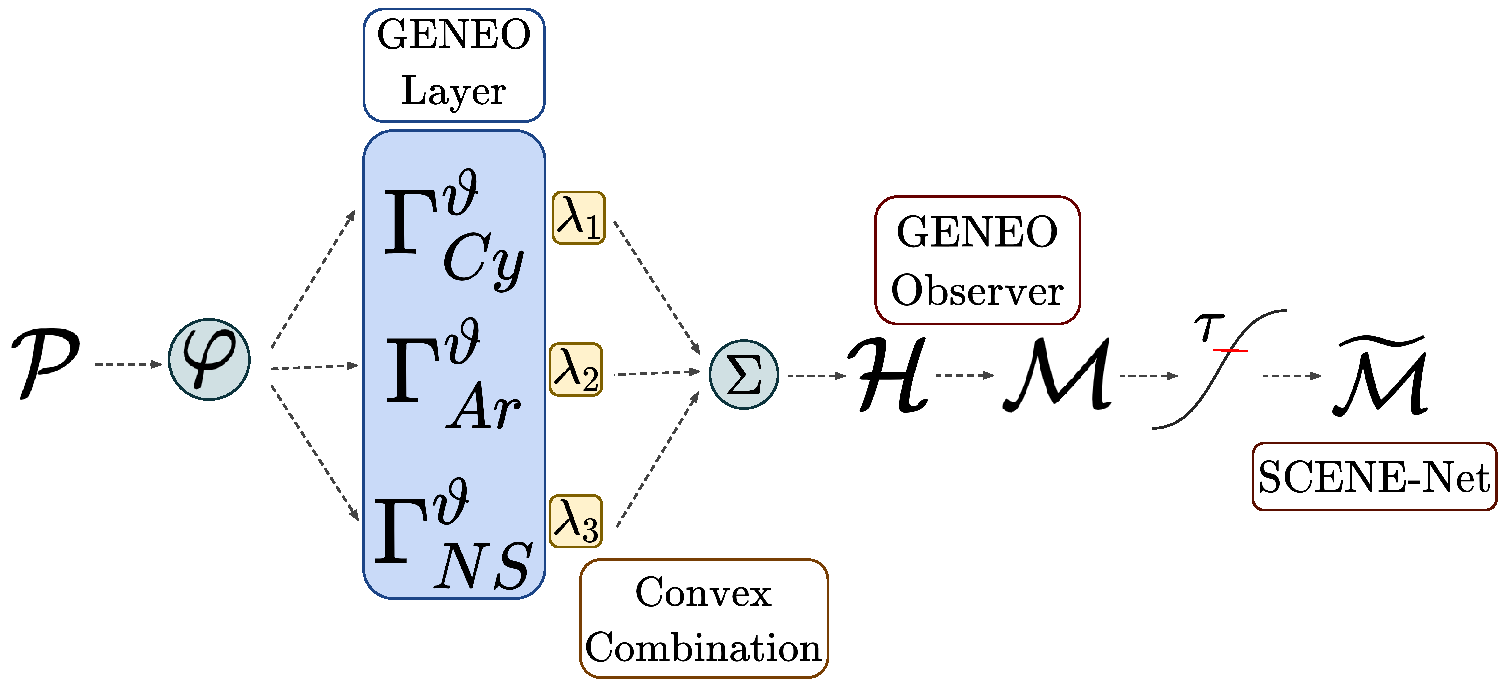
\includegraphics[width=.9\textwidth]{GNet_Overview.pdf}
    \caption{Pipeline of SCENE-Net: an input point cloud  $\mathcal{P}$ is measured according to function $\varphi$ and voxelized. This representation then is fed to a GENEO-layer, where each operator $\Gamma_i^{\vartheta_i}$ separately convolves the input.
    A GENEO observer $\mathcal{H}$ is then achieved by a convex combination of the operators in the GENEO layer.
    $\mathcal{M}$ transforms the analysis of the observer into a probability of belonging to a tower. %
    Lastly, a threshold operation is applied to classify the voxels. Note that this final step occurs after training is completed.
    }
    \label{fig:gnet_overview}
\end{figure}

\subsection{Overview}

%We discretize 3D point clouds as a grid of voxels $\mathcal{P} \in \R^{X\times Y\times Z}$, where $X, Y$ and $Z$ denote the grid's dimensions.
3D Point clouds are generally denoted as $\mathcal{P} \in \R^{N\times (3 + d)}$, where  $N$ is the number of points and $3 + d$ is the cardinality of spatial coordinates plus any point-wise features, such as colors or normal vectors. 
%
%The pipeline of \textbf{SCENE-Net} is illustrated in Fig.~\ref{fig:gnet_overview}. 
%
The input point cloud is first transformed in accordance with a measurement function $\varphi\colon \R^3 \to \{0, 1\}$ that signals the presence of 3D points in a voxel discretization. 
Next, the transformed input is fed to a layer of multiple GENEOs (GENEO-layer), each chosen randomly from a parametric family of operators, and defined by a set of trainable shape parameters $\vartheta$ (Fig.~\ref{fig:gnet_overview}).
%
Such GENEOs are in the form of convolutional operators with carefully designed kernels as described later. Not only is convolution a well-studied operation, but it also offers equivariance w.r.t. translations by definition. 
%
During training, it is not the kernels themselves that are fine-tuned with back-propagation, since this would not preserve equivariance at each optimization step. Instead, the error is propagated to the shape parameters $\vartheta$ of each operator. 
%Cvx combination
Following the GENEO-layer, its set of operators $\Gamma=\{\Gamma_i^{\vartheta_i}\}_{i=1}^K$, 
with shape parameters $\vartheta = \vartheta_1,\dots,\vartheta_k$, 
are combined through convex combination with weights $\lambda = (\lambda_1,\dots,\lambda_k )^T$ by $\observer \colon \mathcal{P} \to \mathcal{P}$ such that
\begin{align}\label{eq:observer}
    \begin{split}
        &\observer(x) = \sum_{i=1}^{K}\lambda_i \Gamma_i^{\vartheta_i}(\varphi)(x)
        %
        %\lambda^T\{\Gamma^\vartheta(\varphi)(x)\}.
    \end{split}
\end{align}
Since the convex combination of GENEOs is also a GENEO~\cite{GENEO19}, $\mathcal{H}$ preserves the equivariance of each operator $\Gamma^\vartheta \in \Gamma$. 
In fact, $\mathcal{H}$ defines a GENEO observer that analyzes the 3D input scenes looking for the geometrical properties encoded in $\Gamma$.
%
The convex coefficients $\lambda$ represent the overall contribution of each operator $\Gamma_i^\vartheta$ to $\mathcal{H}$ to the analysis. 
The parameters grant our model its intrinsic interpretability. They are learned during training and represent geometric properties and the importance of each $\Gamma^\vartheta$ in modeling the ground truth.

%Observer into tower probability
Next, we transform the observer's analysis into a probability of each 3D voxel belonging to a supporting tower as a model $\model \colon \mathcal{P} \to [0, 1]^N$
\begin{align*}
    \begin{split}
        &\model(x) = \bigg(\tanh\Big(\observer(x)\Big)\bigg)_+
    \end{split},
\end{align*}
where $(t)_+ = \max\{0, t\}$ is the rectified linear unit (ReLU).
%The model $\mathcal{M}$ represents the explaination of the observer $H$ into a probability of $x$ being part of a supporting tower.
%Where $(\cdot)_+$ defines ramp function, more commonly known as rectified linear unit (ReLU). 
Negative signals in $\mathcal{H}(x)$ represent patterns that do not exhibit the sought-out geometrical properties. Conversely, positive values quantify their presence.
%
Therefore, $\tanh$ compresses the observer's value distribution into [-1, 1], and the ReLU is then applied to enforce a zero probability to negative signals.
%
%Apply classification threshold
Lastly, a probability threshold $\tau \in [0, 1]$ is defined through hyperparameter fine-tuning and applied to $\mathcal{M}$ resulting in a map $\widetilde{\model} \colon \mathcal{P}\times \R \to \{0, 1\}^N$
\begin{align*}
    \begin{split}
        &\widetilde{\model}(x, \tau) = \Big\{\model(x)\Big\} \geq \tau
    \end{split},
\end{align*}
where $\widetilde{\mathcal{M}}$ denotes the \textbf{SCENE-Net} model.

\subsection{Knowledge Engineering via GENEOs}
%
In this section, we formally define the knowledge embedded in the observer $\mathcal{H}$. The following GENEOs describe power line supporting towers in order to fully discriminate them from their environment.
% During the knowledge engineering phase of building an observer, prior knowledge is defined to formally describe power line supporting towers and fully discriminate them from the surrounding environment.
% %
% The following GENEOs define geometrical properties of supporting towers along with other patterns that should be disregarded by the observer.

\subsubsection{Cylinder GENEO}
The most striking characteristic of supporting towers against the rural environment is their long, vertical and narrow structure. 
As such, their identification is equivariant w.r.t. rotations along the \textit{z-axis} and translations in the \textit{xy} plane, which we encode by the means of a cylinder.

\begin{definition} \label{prop:cylinder}
In order to promote smooth patterns, a cylinder is defined by $g_{Cy}\colon \R^3 \to [0, 1]$:
\begin{align*}
    \begin{split}
        &g_{Cy}(x) = e^{-\frac{1}{2\sigma^2}(\Vert \pi_{-3}(x) - \pi_{-3}(c) \Vert^{2} - r^2 )^2}
    \end{split}
\end{align*}
%
% with $\pi_{-3}$ being a projection function that nullifies the last coordinate of a 3-element vector:
% \begin{align}
%     \begin{split}
%         %&\pi_{-3}\colon \R^3 \to \R^3 \\
%         \pi_{-3}(x) = (\pi_{1}(x), \pi_{2}(x), 0)
%     \end{split}
% \end{align}
where $\pi_{-3}(x) = (\pi_{1}(x), \pi_{2}(x),0)$ and $\pi_i$ defines a projection function of the $i$th element of the input vector. 
\end{definition}
%
Definition~\ref{prop:cylinder} is a smoothed characterization of a cylinder.
The function $g_{Cy}$ defines a smoothed cylinder centered in $c$ by means of a Gaussian function, with the distance between $x$ and the cylinder's radius ($r$) as its mean.
The shape parameters are the Gaussian's standard deviation and $r$, defined as $\vartheta_{Cy} = [r, \sigma]$.

GENEOs act on functions, transforming them to remain equivariant to a specific group of transformations. Our GENEOs act upon $\Phi$, the topological space representing $\mathcal{P}$ with admissible functions $\varphi\colon \R^3 \to \{0, 1\}$. 
Specifically, we work with appropriate $\varphi \in \Phi$ functions that represent point clouds and preserve their geometry. For instance, $\varphi$ can be a function that signals the presence of 3D points in a voxel grid.  
Therefore, the cylinder GENEO $\Gamma_{Cy}^\vartheta$ transforms $\varphi$ into a new function that detects sections in the input point cloud that demonstrate the properties of $g_{Cy}$ and, simultaneously, preserves the geometry of the 3D scene
\begin{align*}
        &\Gamma_{Cy}^\vartheta\colon \Phi \to \Psi, \qquad \psi_{Cy} = \Gamma_{Cy}^\vartheta (\varphi) \nonumber \\
        &\psi_{Cy} (x) = \int_{\R^3} \Tilde{g}_{Cy}(y)\varphi(x - y)dy
        %g_{Cy}(x) - \frac {\int_{C} g_{Cy}(z)dz}{V(C)} ,
\end{align*}

where $\Psi$ is a new topological space that represents $\mathcal{P}$ with functions $\psi\colon \R^3 \to [0, 1]$ and $\Tilde{g}_{Cy}$ defines a normalized Cylinder.
%
The kernel $g_{Cy}$ is normalized to have a zero-sum to promote the stability of the observer.
This way, we encourage the geometrical properties that exhibit the sought-out group of transformations and punish those which do not.
Thus, $\psi_{Cy}(x)$ assumes positive values for 3D points near the radius, whereas negative values discourage shapes that do not fall under the $g_{Cy}$ definition. 
This leads to a more precise detection of the encoded group of transformations. 
% \begin{figure}[tb]
%     \centering
%     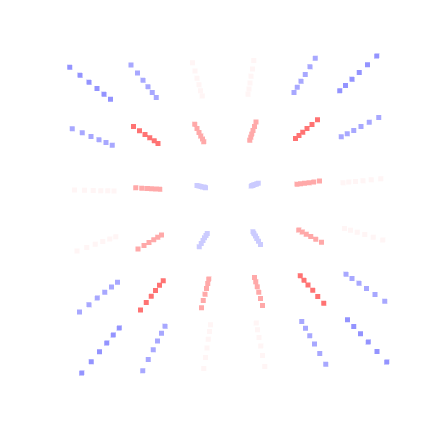
\includegraphics[width=0.42\textwidth]{GENEOs/cylinder.png}
%     \caption{Cylinder kernel computed in a voxel grid. Colored according to weight distribution. Red symbolizes values near 1; Whereas values near -1 are blue; and white is for values close to zero. }
%     \label{fig:cylinder}
% \end{figure}
The cylinder kernel discretized in a voxel grid can be seen in Fig.~\ref{fig:cylinder}.

\subsubsection{Arrow GENEO}
Towers are not the only element in rural environments characterized by a vertical and narrow structure. The identification of trees also shows equivariance w.r.t. rotations along the \textit{z-axis}. 
Therefore, it is not enough to detect the body of towers, we also require the power lines that they support.
To this end, we define a cylinder following the rationale behind the cylinder GENEO with a cone on top of it.
%
This arrow defines equivariance w.r.t. the different angles at which power lines may find their supporting tower.
\begin{definition} \label{prop:arrow}
The function describing the Arrow is defined as $g_{Ar}\colon \R^{3} \to [0, 1]$:

\begin{align*}
    \begin{split}
        &g_{Ar}(x)=
        \twopartdef
        {e^{\frac{-1}{2\sigma^2}(\Vert \pi_{-3}(x) - \pi_{-3}(c) \Vert^{2} - r^2 )^2}}{\pi_3(x) < h}
        {e^{\frac{-1}{2\sigma^2}(\Vert \pi_{-3}(x) - \pi_{-3}(c) \Vert^{2} - (r_c\tan(\beta\pi))^2 )^2}}{\pi_3(x) \geq h}
    \end{split}
\end{align*}
with  $\beta \in [0, 0.5)$ defining the inclination of the cone.
\end{definition}
Definition~\ref{prop:arrow} is a smoothed characterization of a cone on top of a cylinder.
 The radii of the cylinder and cone are defined by $r$ and $r_c$, respectively, with $c$ as their center. Lastly, $h$ defines the height at which the cone is placed on top of the cylinder.
Thus, the shape parameters of the Arrow are defined by the vector $\vartheta_{Ar} = [r, \sigma, h, r_c, \beta].$
%
Lastly, we are also interested that this kernel sums to zero, so we define
% \begin{align}
%     &\Gamma_{Ar}^\vartheta(\varphi)(x) = g_{Ar}(x) - \frac {\int_{C} g_{Ar}(x)dx}{V(C)} 
% \end{align}
\begin{align*}
        &\Gamma_{Ar}^\vartheta\colon \Phi \to \Psi, \qquad \psi_{Ar} = \Gamma_{Ar}^\vartheta (\varphi) \nonumber \\
        &\psi_{Ar} (x) = \int_{\R^3} \Tilde{g}_{Ar}(y)\varphi(x - y)dy,
\end{align*}
where $\Tilde{g}_{Ar}(y)$ represents a normalized Arrow kernel. Its discretization is depicted in Fig.~\ref{fig:arrow}.
% \begin{figure}[tb]
%     \centering
%     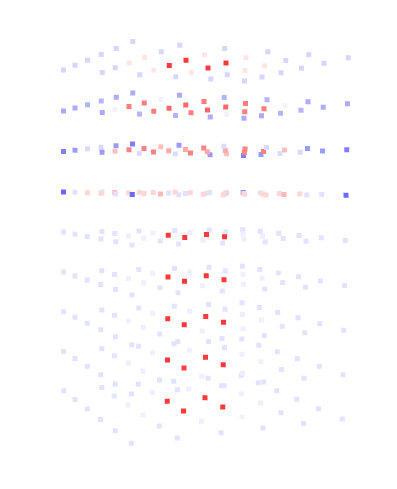
\includegraphics[width=0.35\textwidth]{GENEOs/arrow.png}
%     \caption{Arrow kernel computed in a voxel grid. Colored according to weight distribution}
%     \label{fig:arrow}
% \end{figure}

\subsubsection{Negative Sphere GENEO} 
Detecting power lines does not exclude the remaining objects in the scene whose identification also demonstrates equivariance w.r.t. rotations along the \textit{z-axis}. Tree elements, such as bushes, are especially frequent in the TS40K dataset. 
%
Thus, we designed a negative sphere to diminish their detection and simultaneously punish the geometry of trees.

\begin{definition} \label{prop:ns}
The Negative Sphere $g_{NS}\colon \R^3 \to [-\omega, 1[ $ is defined as
\begin{align*}
    \begin{split}
        &g_{NS}(x) = - \omega e^{\frac{-1}{2\sigma^2}(\Vert x - c\Vert^{2} - r^2 )^2}.
    \end{split}
\end{align*}
with $\omega \in ]0, 1]$ defining a small negative weight that punishes the spherical shape.
\end{definition}
%
Definition~\ref{prop:ns} is a smoothed characterization of a geometric sphere.
The shape parameters of this operator are $\vartheta_{NS} = [r, \sigma, \omega]$.
Since we wish to discourage spherical patterns following the definition of $g_{NS}$, so we do not enforce that its space sums to zero, obtaining
\begin{align*}
        &\Gamma_{NS}^\vartheta\colon \Phi \to \Psi_{NS}, \qquad \psi_{NS} = \Gamma_{NS}^\vartheta (\varphi) \nonumber \\
        &\psi_{NS} (x) = \int_{\R^3} g_{NS}(y)\varphi(x - y)dy.
\end{align*}
where $\Psi_{NS}$ is a topological space containing functions $\psi\colon \R^3 \to [-\omega, 1[$.
Fig.~\ref{fig:neg_sphere} depicts the computation of this kernel in a voxel grid.

\begin{figure}
    \centering
    \subfigure[Cylinder]{ \label{fig:cylinder}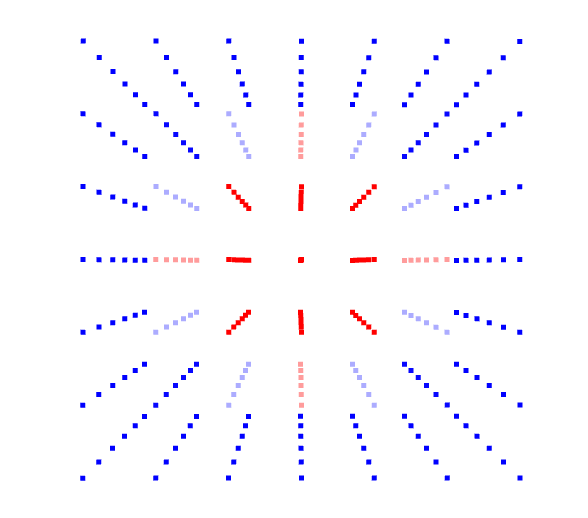
\includegraphics[width=.31\textwidth]{cylinderv2.png}}
    %
    \subfigure[Arrow]{ \label{fig:arrow}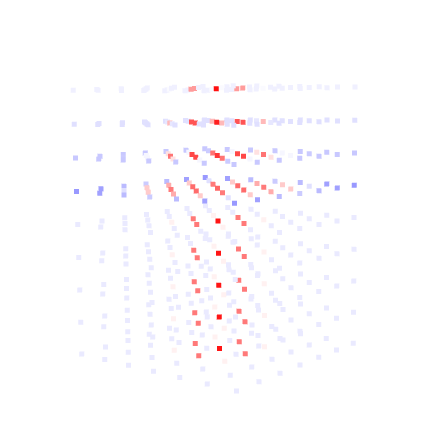
\includegraphics[width=.28\textwidth]{arrowv2.png}}
    %
    \subfigure[Negative Sphere]{ \label{fig:neg_sphere}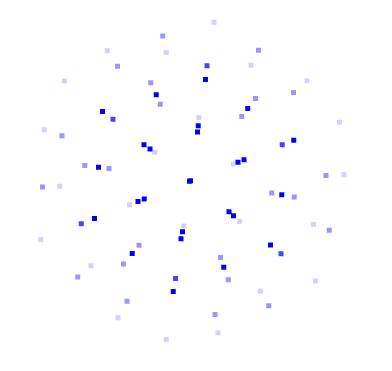
\includegraphics[width=.31\textwidth]{neg_spherev2.png}}
    %
    \subfigure{\centering
    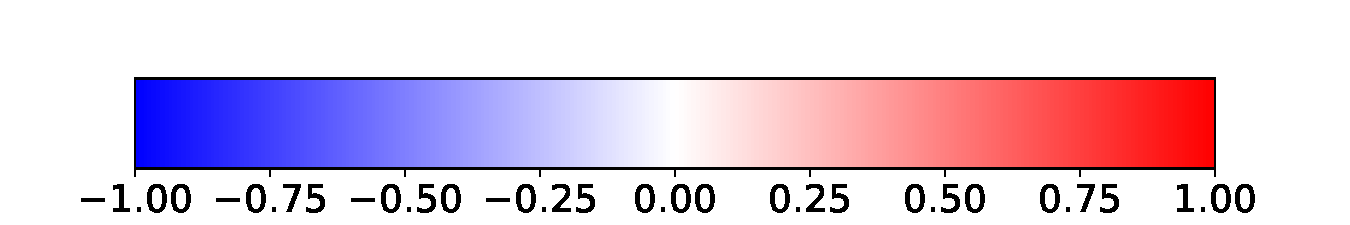
\includegraphics[width=.7\textwidth]{colorbar.pdf}}
\caption{GENEO kernels discretized in a voxel grid and colored according to weight distribution}
\end{figure}

\subsection{GENEO Loss}

The use of GENEOs in knowledge embedding forces our model to uphold the convexity of the observer during training. 
Thus, our problem statement is represented by the following optimization problem
\begin{align*}
    \begin{split}
        \minimize_{\lambda, \vartheta}\quad &\expect_{X, y, \alpha, \epsilon}\bigg\{\mathcal{L}_{seg}(\lambda, \vartheta)\bigg\} \\
        \textrm{s.t} \quad &\vartheta \geq 0 \\ \quad &\lambda^T\textbf{1} = 1\\ \quad &\lambda \geq 0,
    \end{split}
\end{align*}
where the segmentation loss $\mathcal{L}_{seg}$ is defined as
\begin{align*}
    &\mathcal{L}_{seg}(\lambda, \vartheta) =
    f_w(\alpha, \epsilon, y)\Big(\model(X) - y\Big)^2.
    %
    %\\&f_w(\alpha, y) = \frac{f_w''(\alpha, y)}{\frac{1}{N}\sum_{i=1}^{N}f_w''(\alpha, y_i)} \\
    % &\textrm{with,} \quad f_w''(\alpha, y) = \max(1 - \alpha p(y), \epsilon)
\end{align*}
 The loss uses a weighted squared error following the weighting scheme $f_w$ proposed in~\cite{steininger2021density} to mitigate data imbalance. The hyperparameter $\alpha$ emphasizes the weighting scheme, whereas $\epsilon$ is a small positive number that ensures positive weights. Thus, $\expect\{\cdot \}$ represents the expectation of the segmentation loss over the data distribution.
The above constraints ensure that our model $\mathcal{M}$ maintains convexity throughout training, with \textbf{1} denoting a vector composed of entries one.
%
The reparametrization of the hyperparameters $\lambda$ allows us to obtain an equivalent optimization problem, considering $\lambda_k = 1- \sum_{i=1}^{K-1} \lambda_i$, thus obtaining Problem~(\ref{eq:opt2}),
\begin{align}\label{eq:opt2}
    \begin{split}
        \minimize_{\lambda, \vartheta}\quad &\expect_{X, y, \alpha, \epsilon}\bigg\{{\mathcal{L}_{seg}}(\lambda, \vartheta)\bigg\} \\
        \textrm{s.t} \quad &\vartheta \geq 0 \\ \quad &\lambda \geq 0
    \end{split} ,
\end{align}
with one less constraint.
Then, we ensure non-negativity of $\mathcal{M}$'s trainable parameters $\lambda, \vartheta$ by relaxing Problem~\eqref{eq:opt2} and introducing a penalty in the optimization cost definition as
\begin{align}\label{eq:opt_final}
    \begin{aligned}
        \minimize_{\lambda, \vartheta}&\quad \expect_{X, y, \alpha, \epsilon}\bigg\{{\mathcal{L}_{seg}}(\lambda, \vartheta)\bigg\}\; +
        \rho_l\Big( \sum_i^K h(\lambda_i)\Big) + \rho_t\Big( \sum_i^K \sum_j^{T_i} h(\vartheta_{ij})\Big),\\
        % &  \;\;\;\;\;\rho_l\Big(h(\lambda_i)^T\textbf{1}) + \rho_t\Big(h(\vartheta_i)^T\textbf{1}\Big)
    \end{aligned}
\end{align}
where $h(x) = \big( -x\big)_+ $, $\rho_l$ and $\rho_t$ are scaling factors of the negativity penalty $h$, $K$ is the number of GENEO-kernels that composes $\mathcal{M}$ and $T_i$ is the number of shape parameters in $\vartheta_i$.
%
GENEO final loss is formalized in optimization Problem~(\ref{eq:opt_final}). It consists of a data fidelity component (i.e., $\mathcal{L}_{seg}$) and two penalties on negative parameters. 

% \section{TS40K Dataset}

% Electrical companies are responsible for the maintenance and inspection of the transmission system. They deploy low-flying helicopters to scan rural environments, from a BEV perspective, where the electrical grid is located.
% %
% The produced point clouds exhibit different data properties when compared to 3D scenes captured from other viewpoints, such as from a vehicle.
% Namely, they show high point density and no object occlusion, scene elements present homogeneous density no sparsity.
% %
% Then, the acquired 3D data is processed by maintenance personnel. Specifically, seeing as the raw point clouds are quite verbose and mainly encompass campestral areas, data is sectioned into strips of land focused on the transmission system as shown in Figure~\ref{fig:ts40k}. 
% %

% \begin{figure}[h]
%     \centering
%     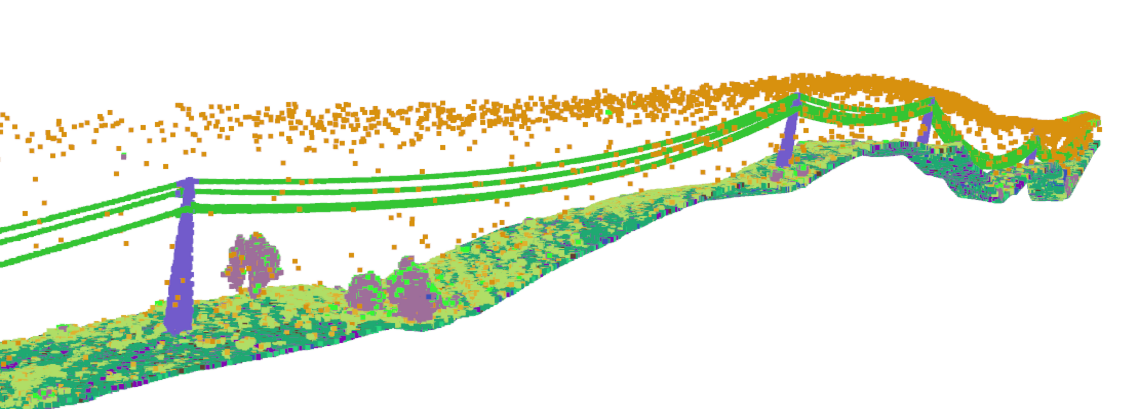
\includegraphics[width=1\textwidth]{data5-5.png}
%     \caption{Visualization of TS40K raw point clouds after segmentation and classification}
%     \label{fig:ts40k}
% \end{figure}

% The raw data is composed of several LiDAR files containing roughly 40 000 kilometers of the above land strips. 3D points therein are labeled with one out of 22 possible classes, such as power lines and their supporting towers, low and medium vegetation, rivers, railroads, human-made structures that do not belong to the transmission network, the ground, optic cables, among others.
% %
% Table~\ref{tab:ts40k_labels} depicts these classes and their density in the dataset. Rail lines and road surface constitute the majority of the dataset (63\%), whereas classes of interest, such as power line supporting towers, make up less than 5\% of the overall data. 


% \begin{table}[]
% \resizebox{\textwidth}{!}{%
% \begin{tabular}{lll|lll}
% \hline
% \textbf{Label} &
%   \textbf{Class} &
%   \textbf{Density(\%)} &
%   \textbf{Label} &
%   \textbf{Class} &
%   \textbf{Density(\%)} \\ \hline
% 0  & Created          & 0               & 11 & Road surface                    & \textbf{18.758} \\
% 1  & Unclassified     & 0.571           & 12 & Overlap points                  & 23.403          \\
% 2  & Ground           & 0.529           & 13 & Medium Reliability              & 0               \\
% 3  & Low vegatation   & 0.681           & 14 & Low Reliability                 & 0               \\
% 4 &
%   Medium vegatation &
%   0.241 &
%   {\color[HTML]{CB0000} 15} &
%   {\color[HTML]{CB0000} Power line support tower} &
%   {\color[HTML]{CB0000} \textbf{0.519}} \\
% 5  & Natural obstacle & 1.069           & 16 & Main power line                 & 0.907           \\
% 6  & Human structures & 0               & 17 & Other power line                & 0.002           \\
% 7  & Low point        & 0.362           & 18 & Fiber optic cable               & 0               \\
% 8  & Model keypoints  & 0               & 19 & Not rated object to be consider & 8.205           \\
% 9  & Water            & 0               & 20 & Not rated object to be ignored  & 0               \\
% 10 & Rail             & \textbf{44.752} & 21 & Incidents                       & 0               \\ \hline
% \end{tabular}%
% }
% \caption{Available classes in the TS40K dataset and their density probabilities. Rail lines and road surface constitute the majority of the dataset (63\%). Whereas our class of interest, power line support tower, only makes up 0.52\%. 
% Moreover, around 40\% of tower points are mislabeled}
% \label{tab:ts40k_labels}
% \end{table}



\section{Experiments}
\label{sec:experiments}
% Section for the interested reader.
%
%% Paragraph template: %%
% Purpose ... Approach. Results (Fig. xx). Interpretation.
% Purpose: Why did we look into this?
% Approach: How did we look into this?
% Results: what are the objective results? What Fig/table evidences them?
% Interpretation: What is the conclusion you reach based on the result. (interpretation touches purpose)
%
% First paragraph: "Lay of the Land"
% - Describe overall aims of paper
% - Introduce shorthands
% - Give an overview of the section argument
In this Section, we assess properties of our model SCENE-Net that help electrical companies in the inspection of power lines: (1) TS40K dataset, (2) training protocol, (3) interpretability of the model, (4) accuracy, (5) robustness to noisy labels, (6) training and inference time, and (7) performance on the SemanticKITTI benchmark.

\subsection{Dataset}

\begin{figure}[h]
\centering
\begin{minipage}[t]{.45\columnwidth}
  \centering
  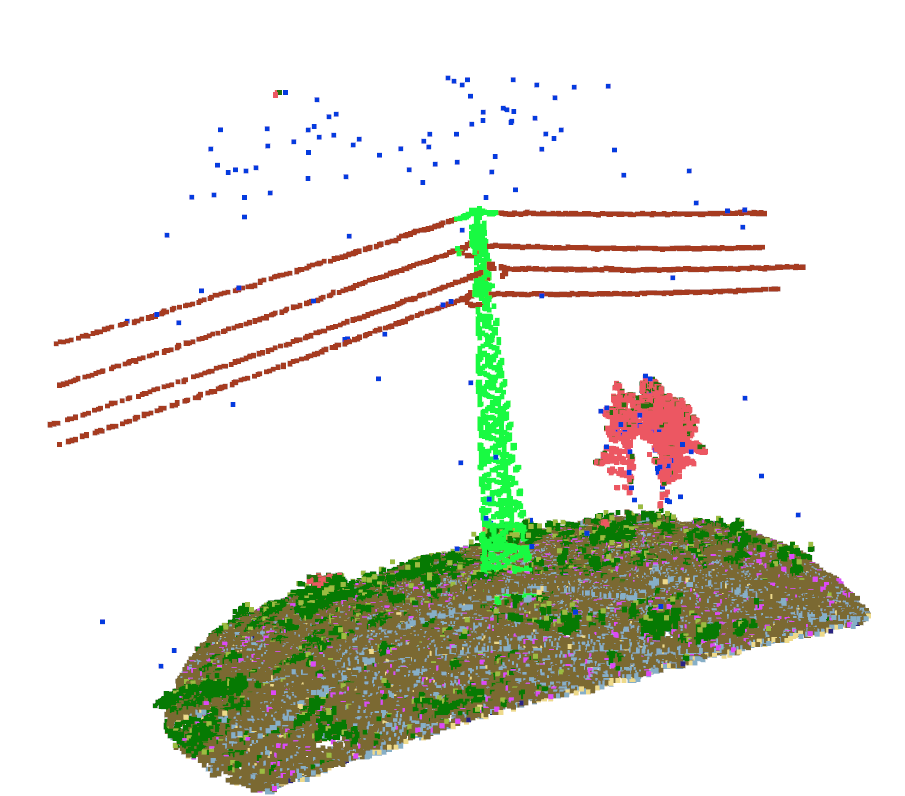
\includegraphics[width=1\columnwidth]{data8.png}
  \caption{Crop sample from the TS40K dataset.}
  \label{fig:crop}
\end{minipage}%
\hfill
\begin{minipage}[t]{.45\columnwidth}
  \centering
  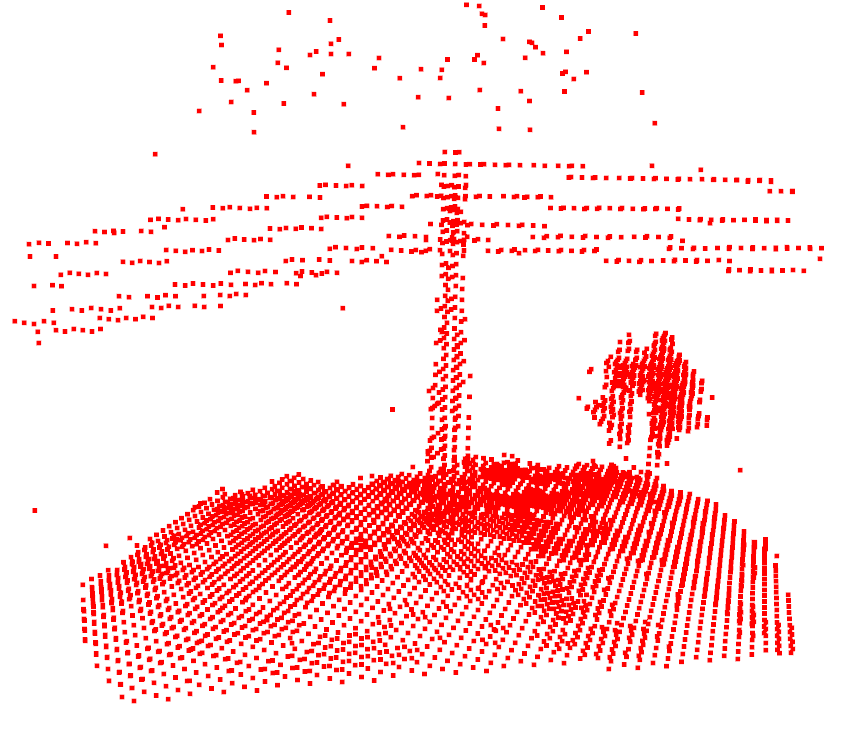
\includegraphics[width=1\columnwidth]{vox64lab.png}
  \caption{Voxelization of sample in Figure~\ref{fig:crop}.}
  \label{fig:vox}
\end{minipage}
\end{figure}

We evaluate the effectiveness of SCENE-Net on the TS40K dataset.
To mitigate the severe data imbalance in our class of interest, we created an ancillary dataset focused on power line-supporting towers with 2823 samples. For each tower in the 3D data, we crop the ground around it with a radius equal to its height.
%
This process introduces bias on classical machine learning agents, such as CNNs.
% One could argue that this process introduces an unnecessary bias on SCENE-Net. That could be the case for classical deep learning agents, seeing as they plainly model their weights to the ground truth (GT) to minimize the training loss.
Contrastingly, SCENE-Net is optimized, after incorporating the appropriate prior knowledge, to detect the chosen features that describe ground-truth. 
A biased training dataset results in an agent tailored to detect supporting towers' geometry. Elements in the 3D scene that do not align with these properties are not signaled by SCENE-Net.
%
Furthermore, we discretize the cropped point clouds with a volume of $64^3$ voxels. If a voxel contains any 3D tower points, it is labeled as a tower voxel, otherwise, it is labeled as a non-tower voxel. This emphasizes the geometry of supporting towers so that they can be better described by SCENE-Net. 
%
To represent the 3D input, all non-empty voxels are given a value of 1. This measurement function preserves the structure of raw point clouds and mitigates the difference in point density between supporting towers and other classes. 
%



\subsection{Training Protocol\label{sec:train_protocol}}

During the end-to-end training process of SCENE-Net, we adopt the following settings:
batch size is 8 for a total of 50 epochs. We employ the RMSProp optimizer with a learning rate of 0.001. The weighting scheme parameters $\alpha$ and $\epsilon$ are set to 5 and 0.1, respectively. While both scaling factors of the non-positive penalty $\rho_l$ and $\rho_t$ are set to 5. The kernel size used to discretize the GENEO operators is $9^3$.
The GENEOs parameters $\vartheta$ are randomly initialized under suitable and positive ranges. While the convex coefficients $\lambda_0,\dots,\lambda_{n-1}$ are randomly initialized in the range $[0, \frac{2}{N-1}]$ to promote a valid convex space for $\mathcal{H}$.
%
To demonstrate that SCENE-Net achieves good results even with fewer data, we use 20\% of the dataset for training, 10\% for validation, and 70\% for testing.
All experiments were conducted on an NVIDIA GeForce RTX 3070 GPU.


\subsection{Interpretability of the trained SCENE-Net: The meaning of the 11 learned parameters}
\label{sec:results-interpretability}
To understand if the model parameters are interpretable, we inspect SCENE-Net's 11 trainable parameters $\vartheta$ and $\lambda$ after training.
% The parameters are grouped by geometrical object, or observer, and jointly combined by their convex combination trainable parameters. 
Each $\vartheta_i \in \vartheta$ holds the learned shape parameters of a geometrical operator $\Gamma_i$, such as their height or radius.
The convex coefficients $\lambda$ weigh each operator $\Gamma_i$ in our model's analysis.
%The geometrical parameters $\vartheta$, such as the heights or radii of geometrical observers that are learned in the training data, and the convex coefficients $\lambda$, that weigh each geometrical observer for the final model. 
For example, we can conclude that the instance $\vartheta_{NS}$ of the Negative Sphere GENEO ($\Gamma_{NS}$) holds a weight of 76.34\% on SCENE-Net's output (Fig.~\ref{fig:interpretable}).
%
The geometric nature of the observer and combination parameters endow intrinsic \textbf{interpretability} to SCENE-Net.  
\begin{figure}
 \centering 
 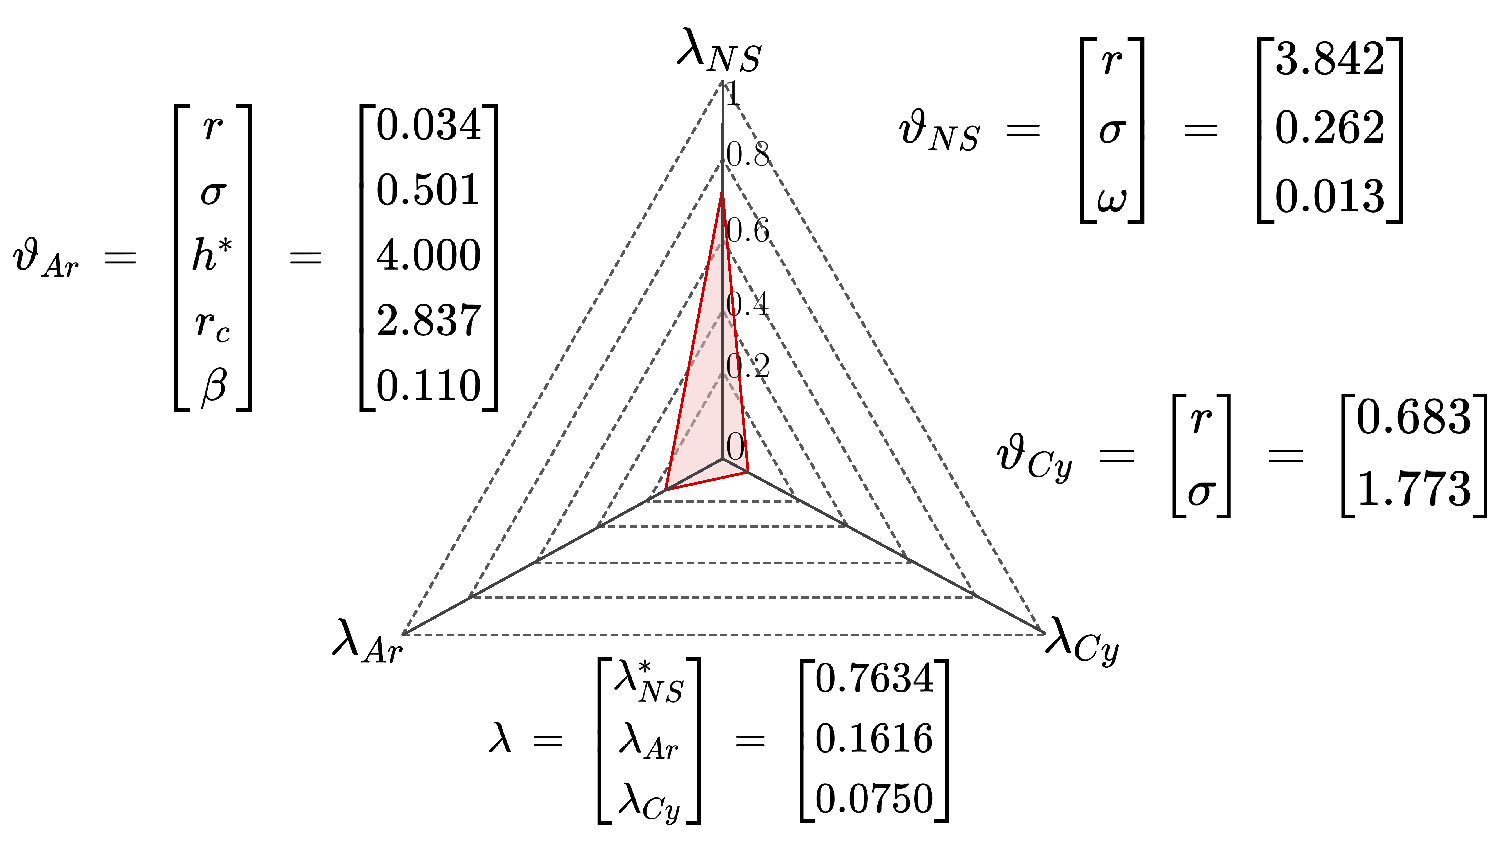
\includegraphics[width=.9\textwidth]{GNet_interpretable.pdf}
 \caption{The trainable parameters of SCENE-Net, $\vartheta$ and $\lambda$. Parameter $h^*$ is not trainable, and $\lambda_{NS}^*$ is defined as a function of the other mixing weights $\lambda_{NS}^* = 1 - \lambda_{Ar} - \lambda_{Cy}$}
 \label{fig:interpretable}
\end{figure}
\subsection{Post-hoc interpretation for specific predictions}
%The geometric operators in SCENE-Net also enable a post-hoc interpretation of SCENE-Net's predictions. 
%
We can correlate the detection of scene elements, such as vegetation, to the contributions of each GENEO. This provides an extra layer of transparency to our model.
%
%For instance, Figure~\ref{fig:posthoc} illustrates the convolution of each GENEO kernel with a TS40K scene.
The Arrow kernel is responsible for the detection of towers, the Cylinder aids this process and diminishes the detection of vegetation, and the Negative Sphere stabilizes the model by balancing contributions of the previous kernels (Fig~\ref{fig:posthoc}). 
\begin{figure}[h]
    \centering
     \subfigure[TS40K scene]{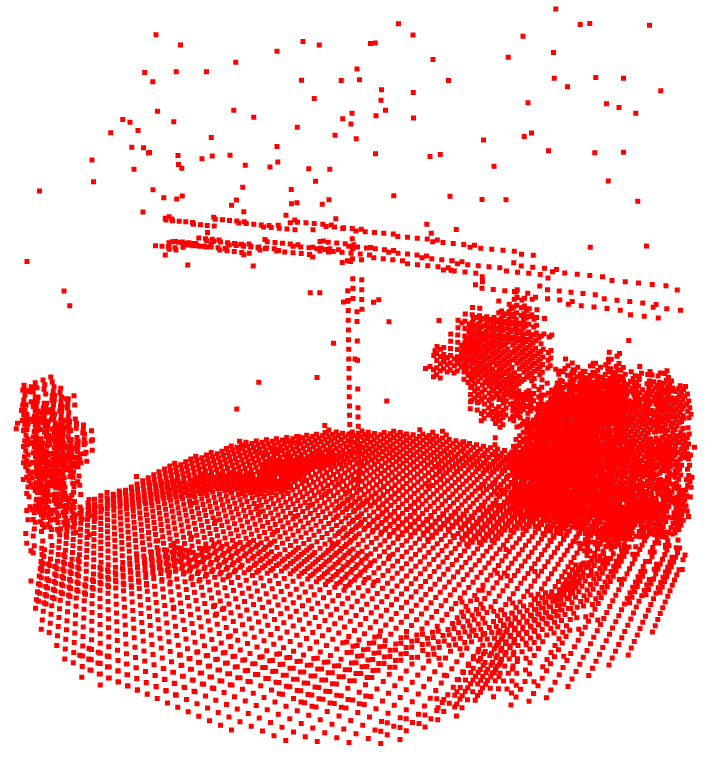
\includegraphics[width=.35\textwidth]{s33.png}}
    %
     \subfigure[Cylinder]
     {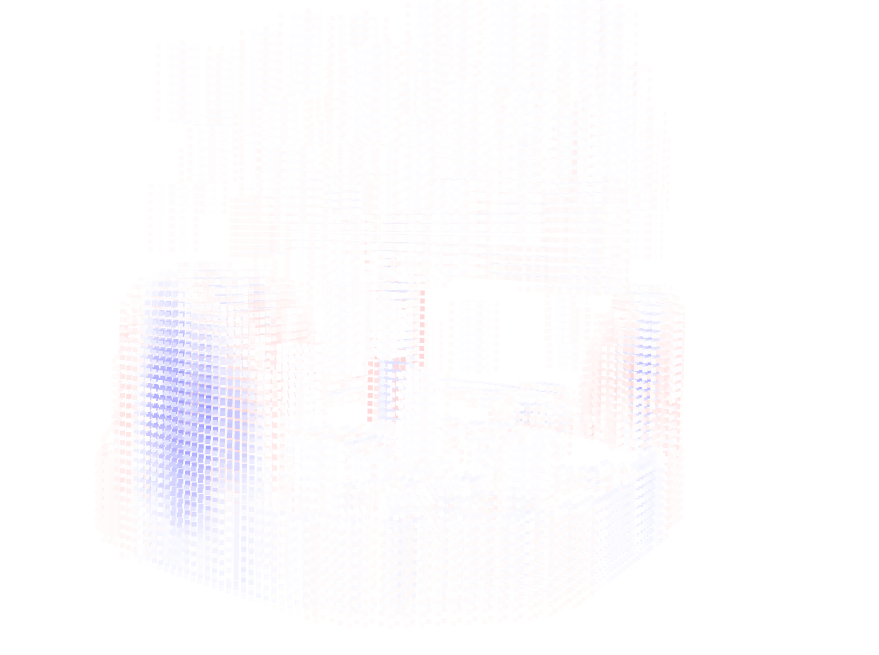
\includegraphics[width=.36\textwidth]{act_cy_s33_v2.png}}
    %
     \subfigure[Arrow]
     {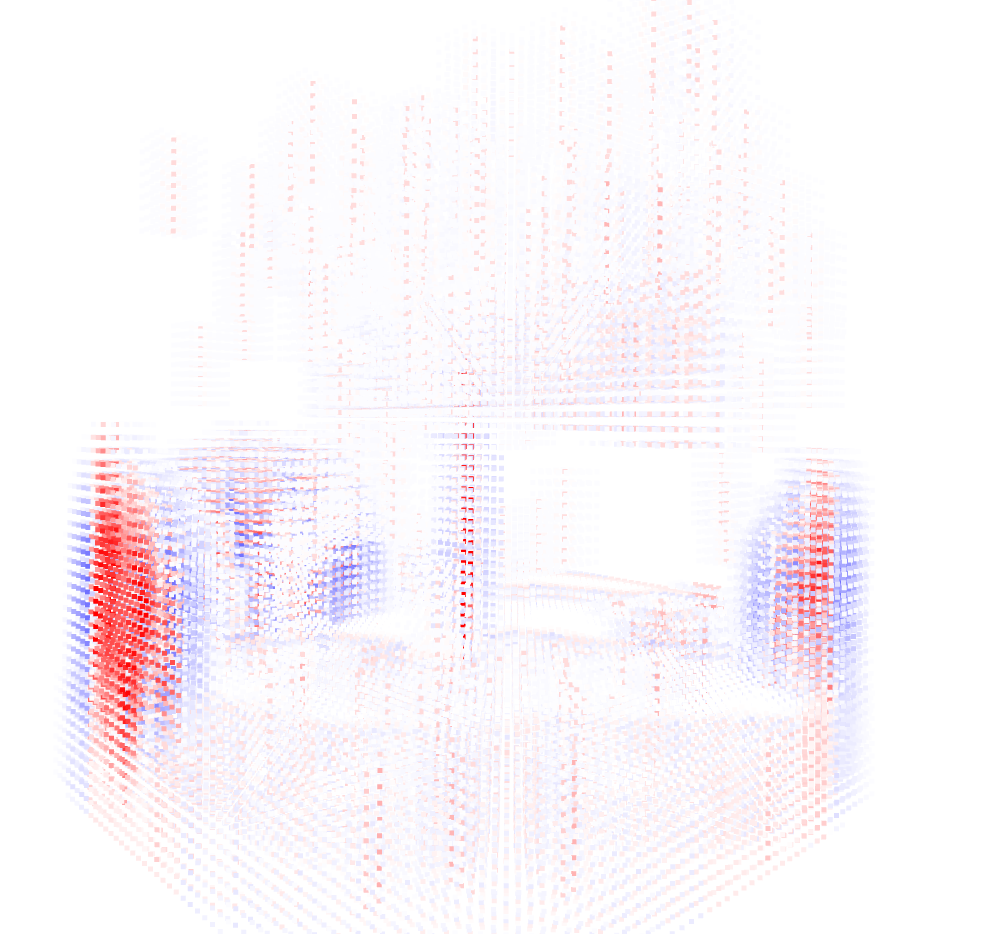
\includegraphics[width=.35\textwidth]{act_arrow_s3_v2.png}}
    %
     \subfigure[Negative Sphere]
     {
\includegraphics[width=.31\textwidth]{act_ns_s33_v2.png}}
    %
     \subfigure
     {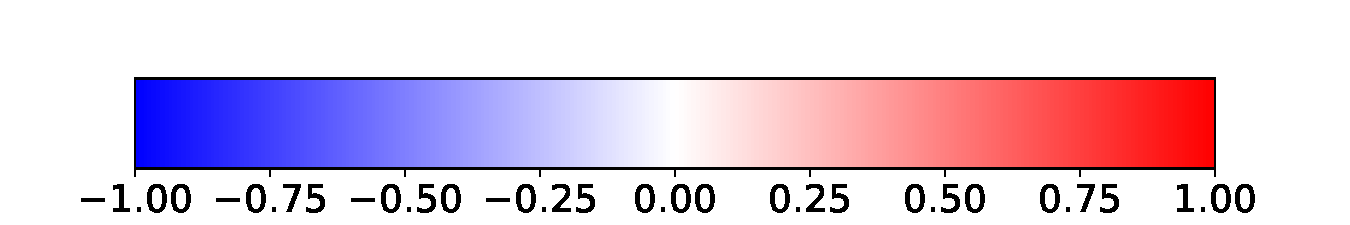
\includegraphics[width=.7\textwidth]{colorbar.pdf}}
     
    \caption{\textit{Post hoc} analysis of SCENE-Net. We can examine the activation of each geometric operator and correlate it to the detection of certain elements in the scene. We see that the Arrow is responsible for the most activation, while the Negative Sphere has a smaller absolute value}
\label{fig:posthoc}
\end{figure}




\subsection{Qualitative accuracy and quantitative metrics: SCENE-Net is more precise in detecting towers than a baseline CNN}
\label{sec:results-accuracy}
To evaluate if SCENE-Net can correctly identify towers in landscapes of the noisy TS40K dataset, we chose the task of 3D semantic segmentation of power line towers. We trained SCENE-Net and a baseline CNN according to the protocol described in Section~\ref{sec:train_protocol}. 
We use a CNN with similar architecture and the same base operator (i.e., convolution) for feature retrieval. 
The main difference is their kernel initialization: SCENE-Net kernels are randomly initialized, but belong to a precise family of operators, while CNN kernels are completely random.
% SCENE-Net  the described observers whereas the kernels of the CNN are randomly initialized. 
%
Running models for 3D point cloud semantic segmentation~\cite{thomas2019kpconv,AF2S3Net,xu2021rpvnet,yan20222dpass} was not done due to their computational requirements.
%
The application penalizes the false positives more, thus we will emphasize Precision. Due to the imbalanced nature of the labels, we measured overall Precision, Recall, and Intersection over Union (IoU). Quantitatively, we observe a lift in Precision of 38\%, and of 5\% in IoU, and a drop of 13\% in Recall (Table~\ref{tab:res_GENEO}). 

\begin{table}[ht!]
\centering
\caption{3D semantic segmentation metrics on TS40K} 
\begin{tabular}{llccc}
\hline
\multicolumn{2}{l}{Method}             & \multicolumn{1}{l}{Precision} & \multicolumn{1}{l}{Recall} & \multicolumn{1}{l}{IoU} \\ \hline
\multicolumn{2}{l}{CNN}                &  0.44 ($\pm$ 0.07)                      & \textbf{0.26} ($\pm$ 0.02)                     & 0.53                   \\
\multicolumn{2}{l}{SCENE-Net} & \textbf{0.82} ($\pm$ 0.08)                     & 0.13 ($\pm$ 0.05)                      & \textbf{0.58}                    \\ \hline
\end{tabular}
\label{tab:res_GENEO}
\end{table}

%
% vxg-128 | CNN | Pre: 0.35 | Rec: 0.21 | IoU: 0.53 | speed: 2.27s/it
% vxg-128 | GNET | Pre: 0.56 | Rec: 0.12 | IoU: 0.55 | speed: 2.03s/it
%
\begin{figure}[t]
 \centering 
 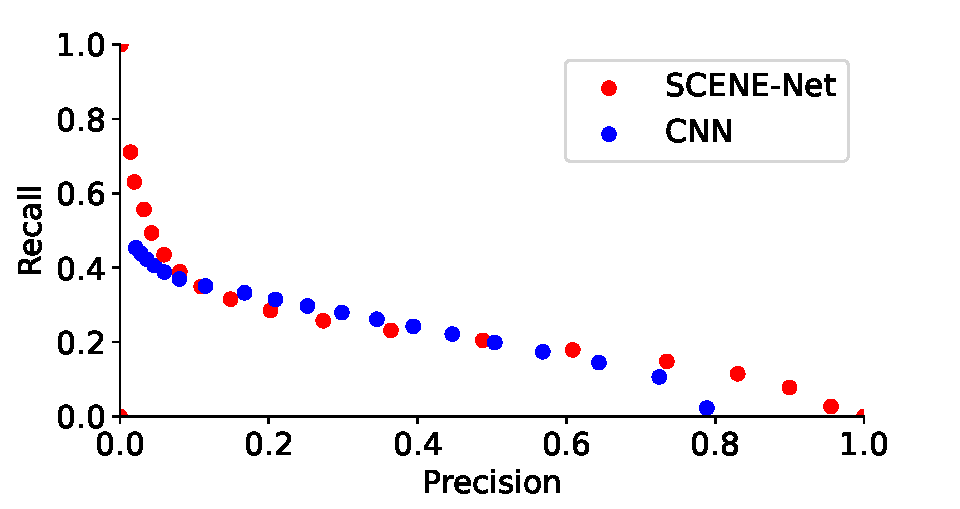
\includegraphics[width=.7\textwidth]{roc_cnn_gnet.pdf}
 \caption{Precision-Recall curve for SCENE-Net and the CNN benchmark, with changing detection threshold. Although our model SCENE-Net has two orders of magnitude fewer parameters than the CNN, it attains a comparable area under the P-R curve}
 \label{fig:recall}
\end{figure}

The lower Recall of SCENE-Net is due to mislabeled points (Figs.~\ref{fig:intro_fig} and \ref{fig:robustness}),  and our choice to privilege Precision over Recall, in view of the fact that the Precision -- Recall curve is slightly better for SCENE-Net (Fig~\ref{fig:recall}).

\subsection{SCENE-Net is robust to noisy labels}
\label{sec:results-robust}
It is important to assess the resilience to noisy labels in the ground-truth (GT) since 50\% of 3D points labelled as supporting tower in the TS40K dataset are, in truth, patches of ground and road surface.
These examples are abundant in the dataset and SCENE-Net is able to recover the body of the tower without detecting ground and power line patches that are mislabeled as tower (Fig.~\ref{fig:robustness}). 
Most noisy labels on this kind of dataset are due to annotation excess around the object of interest and are not randomly distributed. These consistently incorrect labels entail low Recall values (Tab.~\ref{tab:res_GENEO}).
\begin{figure}[t]
\centering
    \subfigure[TS40K scene]
    {\label{fig:robust_input} 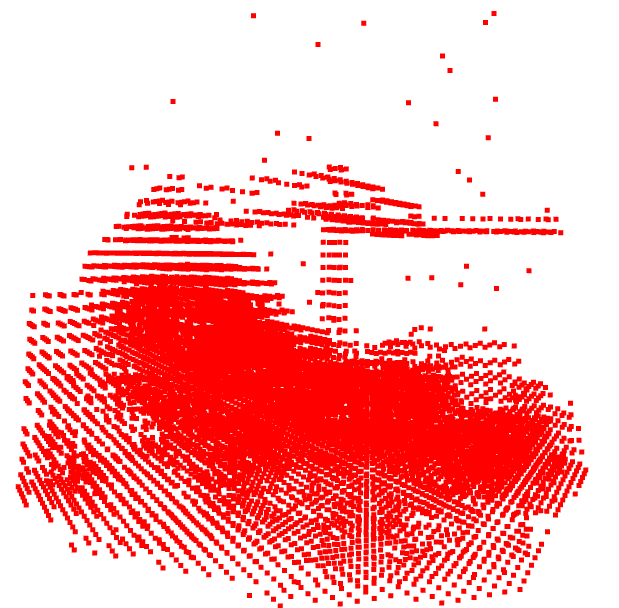
\includegraphics[width=.5\textwidth]{robust_input.png}}
    %
    \subfigure[SCENE-Net prediction against the GT]
     {\label{fig:robust_pred}
     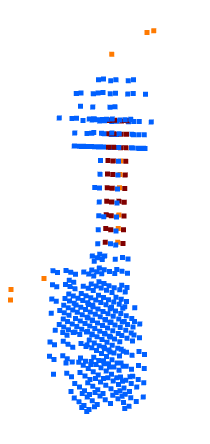
\includegraphics[width=.25\textwidth]{robust_pred.png}}
    %
    \subfigure
     {
\includegraphics[width=.5\textwidth]{color_code_v2.pdf}}
    %
    \caption{SCENE-Net is robust against mislabeled data. Fig.~\ref{fig:robust_pred} compares the prediction of SCENE-Net against the ground truth in Fig.~\ref{fig:robust_input}. SCENE-Net detects the body of the tower, ignoring the patch of ground mislabeled as a tower}
\label{fig:robustness}
\end{figure}


\subsection{SCENE-Net has low data requirements and has modest training time in common hardware}
\label{sec:results-time-efficiency}

The design of SCENE-Net embedded with GENEO observers culminates in a model with 11 meaningful trainable parameters. 
%
This enables the use of common hardware (see Section~\ref{sec:train_protocol} for hardware specs) and a low data regime to train our model.  
%
The results reported in table~\ref{tab:sota_perf} were achieved with 5\% of the \textit{SemanticKITTI} training set. Training SCENE-Net with 50\% and 100\% of the available training data leads to a variation of 0.5\% in pole IoU performance.
%
Moreover, the number of parameters of SCENE-Net remains unchanged regardless of kernel size, whereas in traditional models, such as the baseline CNN with 2190 parameters, the number of parameters grows exponentially with larger kernel sizes.

% To assess if the models can be used 
% in the utility company, we computed the average training and inference times of both the CNN and SCENE-Net (see Supplementary Material for hardware specs). Only one in five trained CNNs returns non-zero predictions. Each training session (50 epochs) takes on average 85~min for a trained SCENE-Net and a CNN. In inference, SCENE-Net takes 20~ms while the CNN takes 43~ms, less 23~ms per inference. The CNN has 2190 trainable parameters, whereas SCENE-Net has 11. 
% The difference in trainable parameters grows exponentially with larger kernel sizes since SCENE-Net has 11 parameters regardless of kernel size.
% %
% % Running models for 3D point cloud semantic segmentation~\cite{thomas2019kpconv,AF2S3Net,xu2021rpvnet,yan20222dpass} was not done due to their computational requirements.
% Training times allow SCENE-Net to be retrained from scratch in less than 90~min. The CNN is also computable, taking on average 8~h to obtain a useful model.



\subsection{SCENE-Net on the SemanticKITTI: an efficient model for low-resource contexts}


In Table~\ref{tab:sota_perf}, we present a comprehensive comparison of the performance of SCENE-Net against state-of-the-art models for the task of 3D semantic segmentation on the \textit{SemanticKITTI} benchmark, specifically in terms of pole IoU, number of parameters, and the ratio of pole IoU to number of parameters.
%
For this problem, we add to the GENEO loss in~(\ref{eq:opt_final}) the Tversky loss~\cite{salehi2017tversky} to boost IoU performance of SCENE-Net:
\begin{align*}
    \mathcal{L}_{Tversky}(y, \hat{y}) = 1 - \frac{y\hat{y} + \delta}{y\hat{y} + \alpha(\textbf{1} - y)\hat{y} + \beta y (\textbf{1} - \hat{y}) + \delta}
\end{align*}

where $y$, $\hat{y}$ are the ground-truth and model prediction, $\alpha, \beta > 0$  are the penalty factors for false positives and false negatives respectively, and $\delta > 0$ is a smoothing term.

The comparison results demonstrate that SCENE-Net is a highly efficient model in terms of its parameter contribution. Our model has the lowest number of parameters, with at least a 5-order magnitude difference from the other models. 
%
SCENE-Net also has the highest ratio of pole IoU to a number of parameters, indicating that it can achieve a high level of performance with a minimal number of parameters. 
%
Although SCENE-Net does not achieve the highest pole IoU performance, it is somewhat on par with state-of-the-art models. 
%
Additionally, SCENE-Net provides intrinsic geometric interpretability and resource efficiency, which makes it a valuable model in high-risk tasks that require trustworthy predictions and good performance but have limited data and computing power.
%
% Considering this, in addition to our strong geometric interpretability and resource efficiency, SCENE-Net guarantees trustworthy predictions for high-risk tasks while maintaining performance on par with state-of-the-art models in 3D segmentation of pole-like structures. 

% Only approaches with their number of parameters available are compared.
\begin{table}[ht]
\centering
\caption{Semantic segmentation on \textit{SemanticKITTI}, only methods that report the parameter count were included. Large models are included for comparison but cannot be used in low-resource contexts. Parameter efficiency is $\frac{\textrm{Pole IoU}}{\textrm{log \#Parameters}}$}
\label{tab:sota_perf}
%\resizebox{\linewidth}{!}{%
\begin{tabular}{cccc}
\hline
\multicolumn{1}{c}{Method} &
  \multicolumn{1}{c}{\begin{tabular}[c]{@{}c@{}}Pole\\ IoU\end{tabular}} &
  \multicolumn{1}{c}{\begin{tabular}[c]{@{}c@{}}\#Parameters\\ (M)\end{tabular}} &
  \multicolumn{1}{c}{\begin{tabular}[c]{@{}c@{}}Parameter \\ Efficiency\end{tabular}} \\ \hline
PointNet++~\cite{qi2017pointnet++}                & 16.9          & 1.48        & 1.19            \\
TangentConv~\cite{tatarchenko2018tangent}               & 35.8          & 0.4   & 2.77            \\
KPConv~\cite{thomas2019kpconv}                    & 56.4          & 14.9        & 3.41            \\
RandLA-Net~\cite{hu2020randla}                & 51.0          & 1.24            & 3.63            \\
RPVNet~\cite{xu2021rpvnet}                    & \textbf{64.8} & 24.8            & 3.80            \\
SparseConv~\cite{graham20183d}                    & 57.9          & 2.7         & 3.91            \\
JS3C-Net~\cite{yan2021sparse}                  & 60.7          & 2.7            & 4.09            \\
SPVNAS~\cite{tang2020searching}                    & 64.3          & 12.5       & 4.62            \\
\textbf{SCENE-Net (Ours)}                      & 57.5      & \textbf{1.1e-5}    & \textbf{23.98} \\ \hline
\end{tabular}%
%}
\end{table}



\begin{figure}[t]
 \centering 
 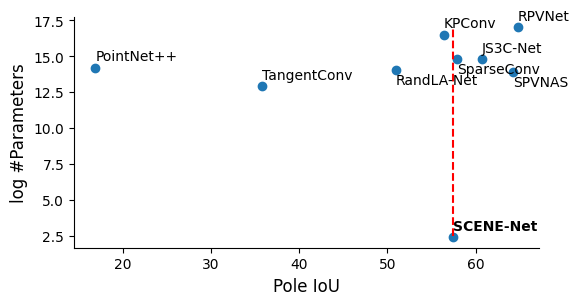
\includegraphics[width=.7\textwidth]{semKITTI_perf.png}
 \caption{Semantic Segmentation results on the \textit{SemanticKITTI} benchmark. Log scale is used for more intelligible comparison}
 \label{fig:semK_perf}
\end{figure}

\begin{figure}[t]
\centering
    \subfigure[\textit{SemanticKITTI} scene]
    {\label{fig:semK_input} 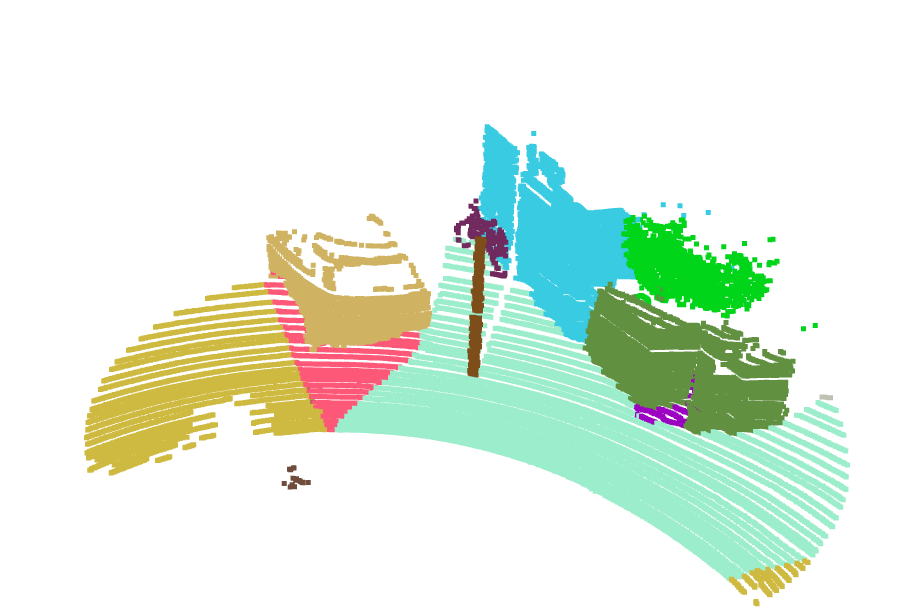
\includegraphics[width=.45\textwidth]{input_7897.png}}
    %
    \subfigure[SCENE-Net prediction against the GT]
     {\label{fig:semK_pred}
     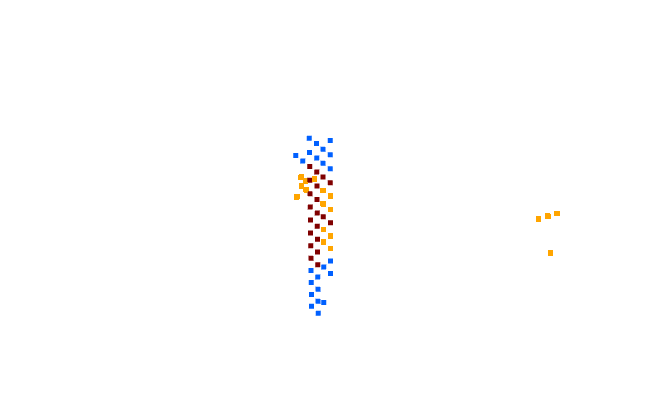
\includegraphics[width=.5\textwidth]{pred_7897.png}}
    %
    \subfigure
     {
\includegraphics[width=.5\textwidth]
     {color_code_v2.pdf}}
    %
    \caption{Qualitative results of SCENE-Net on \textit{SemanticKITTI} for pole detection. Fig.~\ref{fig:semK_pred} compares the prediction of SCENE-Net against the ground truth in Fig.~\ref{fig:semK_input}. SCENE-Net detects the body of the pole while disregarding the rest of the 3D scene}
\label{fig:semK_qualitative}
\end{figure}








\subsection{Ablation Studies}

\begin{table}[t]
\centering
\caption{Ablation Study of SCENE-Net on TS40K validation set.}
%\resizebox{\columnwidth}{!}{%
\begin{tabular}{cl|ccc|ccc}
\hline
\multicolumn{2}{c|}{Model} & Cylinder & Arrow & Neg. Sphere & Precision & Recall & IoU  \\ \hline
\multicolumn{2}{c|}{A}     & 1        & 0    & 0           & 0         & 0      & 0 \\
\multicolumn{2}{c|}{B}     & 0        & 1    & 0           & 0         & 0      & 0 \\
\multicolumn{2}{c|}{C}     & 1        & 0    & 1           & 0.34      & 0.01   & 0.12 \\
\multicolumn{2}{c|}{D}     & 0        & 1    & 1           & 0.13      & 0.01   & 0.08 \\
\multicolumn{2}{c|}{{\color[HTML]{000000} \textbf{E (Ours)}}} &
  {\color[HTML]{000000} \textbf{1}} &
  {\color[HTML]{000000} \textbf{1}} &
  {\color[HTML]{000000} \textbf{1}} &
  {\color[HTML]{000000} \textbf{0.82}} &
  {\color[HTML]{000000} \textbf{0.13}} &
  {\color[HTML]{000000} \textbf{0.58}} \\
\multicolumn{2}{c|}{F}     & 2        & 2    & 2           & 0.56      & 0.16   & 0.53 \\
\multicolumn{2}{c|}{G}     & 3        & 3    & 3           & 0.37      & 0.22   & 0.56 \\ \hline
\end{tabular}%
%}
\label{tab:ablation}
\end{table}

In this section, we conduct ablation studies on SCENE-Net's architecture, specifically on the number of instances of each GENEO. All ablated models were tested on the TS40K validation set.
%
Table~\ref{tab:ablation} shows the following results:
Models A and B are each equipped with a single GENEO, demonstrating an overall poor performance. The Negative Sphere (NS) GENEO proved essential for our observer to disregard arboreal elements in the scene. 
Models C and D study if employing the Cylinder or Arrow combined with NS is enough to analyze the TS40K scenes.
However, SCENE-Net's architecture (model E) yields better results.
Lastly, models F and G test the use of multiple instances of each GENEO, however, this proved to decrease performance when compared to model E.

\subsection{SCENE-Net inference in high resolution, when trained with low-resolution kernel sizes}
\label{sec:results-resolution}
One of the issues of voxel-based models is the computational cost of  3D convolutions with large kernels and high-resolution voxel grids. Here, a CNN architecture leads to an exponential increase in training time.
SCENE-Net has a continuous functional observer of the raw input providing an analysis of its components.
Unlike traditional models, this definition is \textbf{independent} from the input size as well as its own discretization (kernel size). In this experiment, we trained SCENE-Net with voxel grids of $64^3$ and then applied to higher resolutions, such as $128^3$, with good qualitative results (Fig.~\ref{fig:vxg128}). 
% %
% The kernel size used to discretize the operators can be fine-tuned to enhance performance (Tab.~\ref{tab:kernel_sizes}).
%
%
%Conversely, SCENE-Net's architecture is straightforward, demonstrates efficient training times with fewer data required and can analyze higher-resolution voxel grids without the computational burden of training the model with those resolutions.
\begin{figure}[t]
\centering
    \subfigure[Sample discretized in a $128^3$ grid]
    {\label{fig:128_input}
    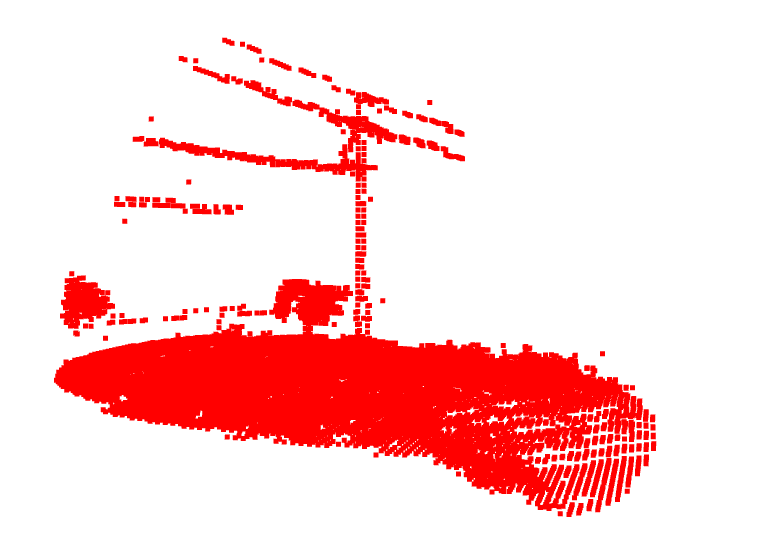
\includegraphics[width=.45\columnwidth]
    {128_s1.png}}
    %
    \subfigure[SCENE-Net prediction against the GT]
    {\label{fig:128_pred}
    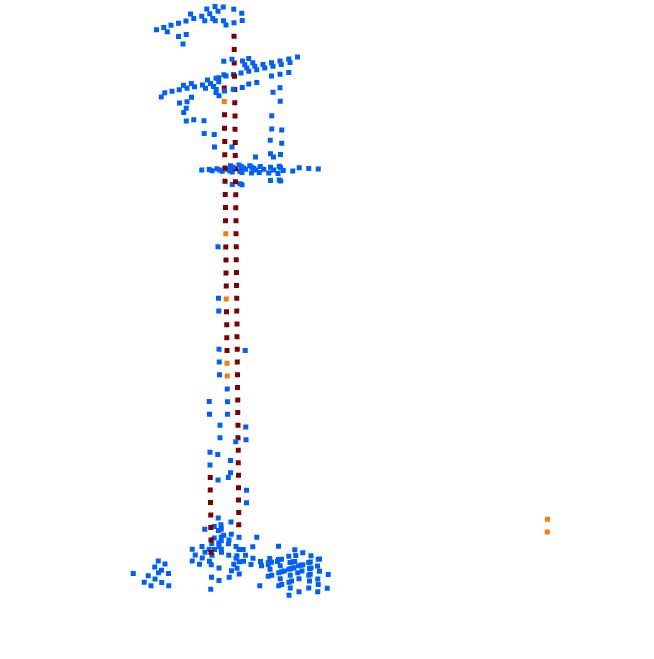
\includegraphics[width=.39\columnwidth]
    {128_gnet_s1.png}}
    %
    \subfigure
    {
\includegraphics[width=.5\columnwidth]
    {color_code_v2.pdf}}
    %
    \caption{SCENE-Net is independent of the input and kernel size. Our model was trained with voxel grids of shape $64^3$ and kernel size $9^3$. Fig.~\ref{fig:128_pred} shows SCENE-Net's prediction against the ground truth of the $128^3$ input grid in Fig.~\ref{fig:128_input} using a kernel-size of $12\times5\times5$.  
}
\label{fig:vxg128}
\end{figure}

% \begin{table}[ht]
%     \centering
%     \caption{Performance of SCENE-Net with different kernel sizes on TS40K. SCENE-Net is trained with a kernel size of $9^3$, which is later fine-tuned to find the sweet spot between Precision and Recall.\\}
%     \begin{tabular}{ccccc}
%     \hline
%     \multicolumn{2}{l}{Kernel-size}             & \multicolumn{1}{l}{Precision} & \multicolumn{1}{l}{Recall} & \multicolumn{1}{l}{IoU} \\ \hline
%     \multicolumn{2}{c}{$9\times9\times9$}                &  0.37 ($\pm$ 0.02)                      & \textbf{0.22} ($\pm$ 0.01)                    & 0.58                  \\
%     \multicolumn{2}{c}{$9\times5\times5$} & \textbf{0.68} ($\pm$ 0.08)                     & 0.16 ($\pm$ 0.05)                     & \textbf{0.58}                    \\ \hline
%     \end{tabular}
%     \label{tab:kernel_sizes}
% \end{table}

\subsection{Template Matching Comparison}

Template matching offers a direct approach to pattern detection by measuring the relation between the input data and a specific pattern of interest. 
Since we define the properties that constitute supporting towers, a comparison between SCENE-Net and this method is reasonable.

Our model combines GENEOs through convex combination and all shape parameters and convex coefficients are found through backpropagation, creating an aggregated GENEO operator - a data observer for composite shape signatures (e.g., cylinder+arrow+negative sphere).
In geometrical methods, such as template matching, this composition is not trivial.
Employing template matching on 3D data is slow, and the parameter initialization (e.g., a Cylinder radius) is a crucial step.
In addition, template matching is not directly applicable to some patterns, e.g., the Neg. Sphere, as it tries to diminish the activation of specific elements. 
We tested template matching of the TS40K with a Cylinder (the same definition used in SCENE-Net) with a radius equal to the average tower radius in the training set. It runs for 12 hours on the validation set of TS40K with an average precision (AP) of 0.001, while SCENE-Net’s AP = 0.2.




\section{Discussion}

% 1. Reiterate narrow problem
% 2. summarize key contributions
% 3. Describe most important interpretations
% 4. State immediate potential implications



Traditional companies, like utilities, need a resource-efficient, responsible application of ML models for the segmentation of real-world point clouds, e.g., for inspecting thousands of kilometers of a power grid.
%
In this paper, we present SCENE-Net, a low-resource white-box model for 3D semantic segmentation. Our approach offers a unique combination of intrinsic geometric interpretability, resource efficiency, and on-par state-of-the-art performance.
%
\paragraph*{Limitations}
Our model prioritizes transparency and performance over broader applicability while allowing a flexible extension.
In this paper, we segmented pole-like structures. State-of-the-art methods often show similar trade-offs, for example, 3D semantic segmentation models are tailored for autonomous driving~\cite{yan2021sparse,xu2021rpvnet}.
SCENE-Net requires a knowledge engineering phase that is not necessary for black-box models.
%
Despite these limitations, we believe that the transparency and efficiency of SCENE-Net make it a valuable tool for high-stakes applications.
%
To detect other shapes, other geometrical observers have to be created. 
As the convex combination of GENEOs is a GENEO, this problem is mitigated by creating a library of primary shapes to be combined to form more complex geometrical structures. 
This is relevant follow-up work, but out of the scope of this paper.
%
Multiclass and multilabel segmentation can be achieved by combining different binary class segmentation models.
%
\paragraph*{Impact}
%We focused on simple signature shapes: the cylinder, arrow and negative sphere. To improve on metrics we could add complex invariant shapes finely describing properties of interest. Here we would pay the price of eliciting detailed properties and narrowing the application field of the model.
%
%
From our experience deploying SCENE-Net within a utility company, low-resource transparent systems can critically help human decision-making---here, by facilitating fast and careful inspection of power lines with interpretable signals of observed geometrical properties. With only three observers and 11 meaningful trainable parameters, SCENE-Net can help reduce the risk of power outages and forest fires by learning from data.




\bibliographystyle{siamplain}
\bibliography{references}


\end{document}
